\section{Update with 2017 data-taking periods}
\label{sec:strong:r21}

The mild excess observed in the multi-bin region SR-0L-HH motivated checking the results with the 2017 data-taking periods 
as soon as they have become available. 
The analysis has been reproduced with all the data collected by the \gls{atlas} experiment in 2015, 2016 and 2017, 
for a total integrated luminosity of 79.8 \ifb. 
Both the cut-and-count and multi-bin regions have been updated in Ref. \cite{ATLAS-CONF-2018-041}, 
but in this section we present only the results 
of the multi-bin regions, since the main purpose is the follow up of the excess in the analysis of the 2015-2016 data.
Differences in the object definition that occurred due to a change in the \gls{atlas} software release between the 
two analyses are not discussed in this section and do not impact sensibly the physics results, more details can be found 
in Ref. \cite{ATLAS-CONF-2018-041}.


\subsection{Results}

The results of the fit in the \glspl{cr} extrapolated to the \glspl{vr} and \glspl{sr} are shown in Figures 
\ref{fig:pullVR_R21} and \ref{fig:pullSR_R21} respectively. 
We can see that there is good agreement with the predicted background in the \glspl{vr}, and the \glspl{vr} do now show any 
significant deviation from the expectations. 
In particular, the excess in SR-0L-HH is no longer present. 

%\begin{figure}[htbp]
%	\centering
%	\subfigure[]{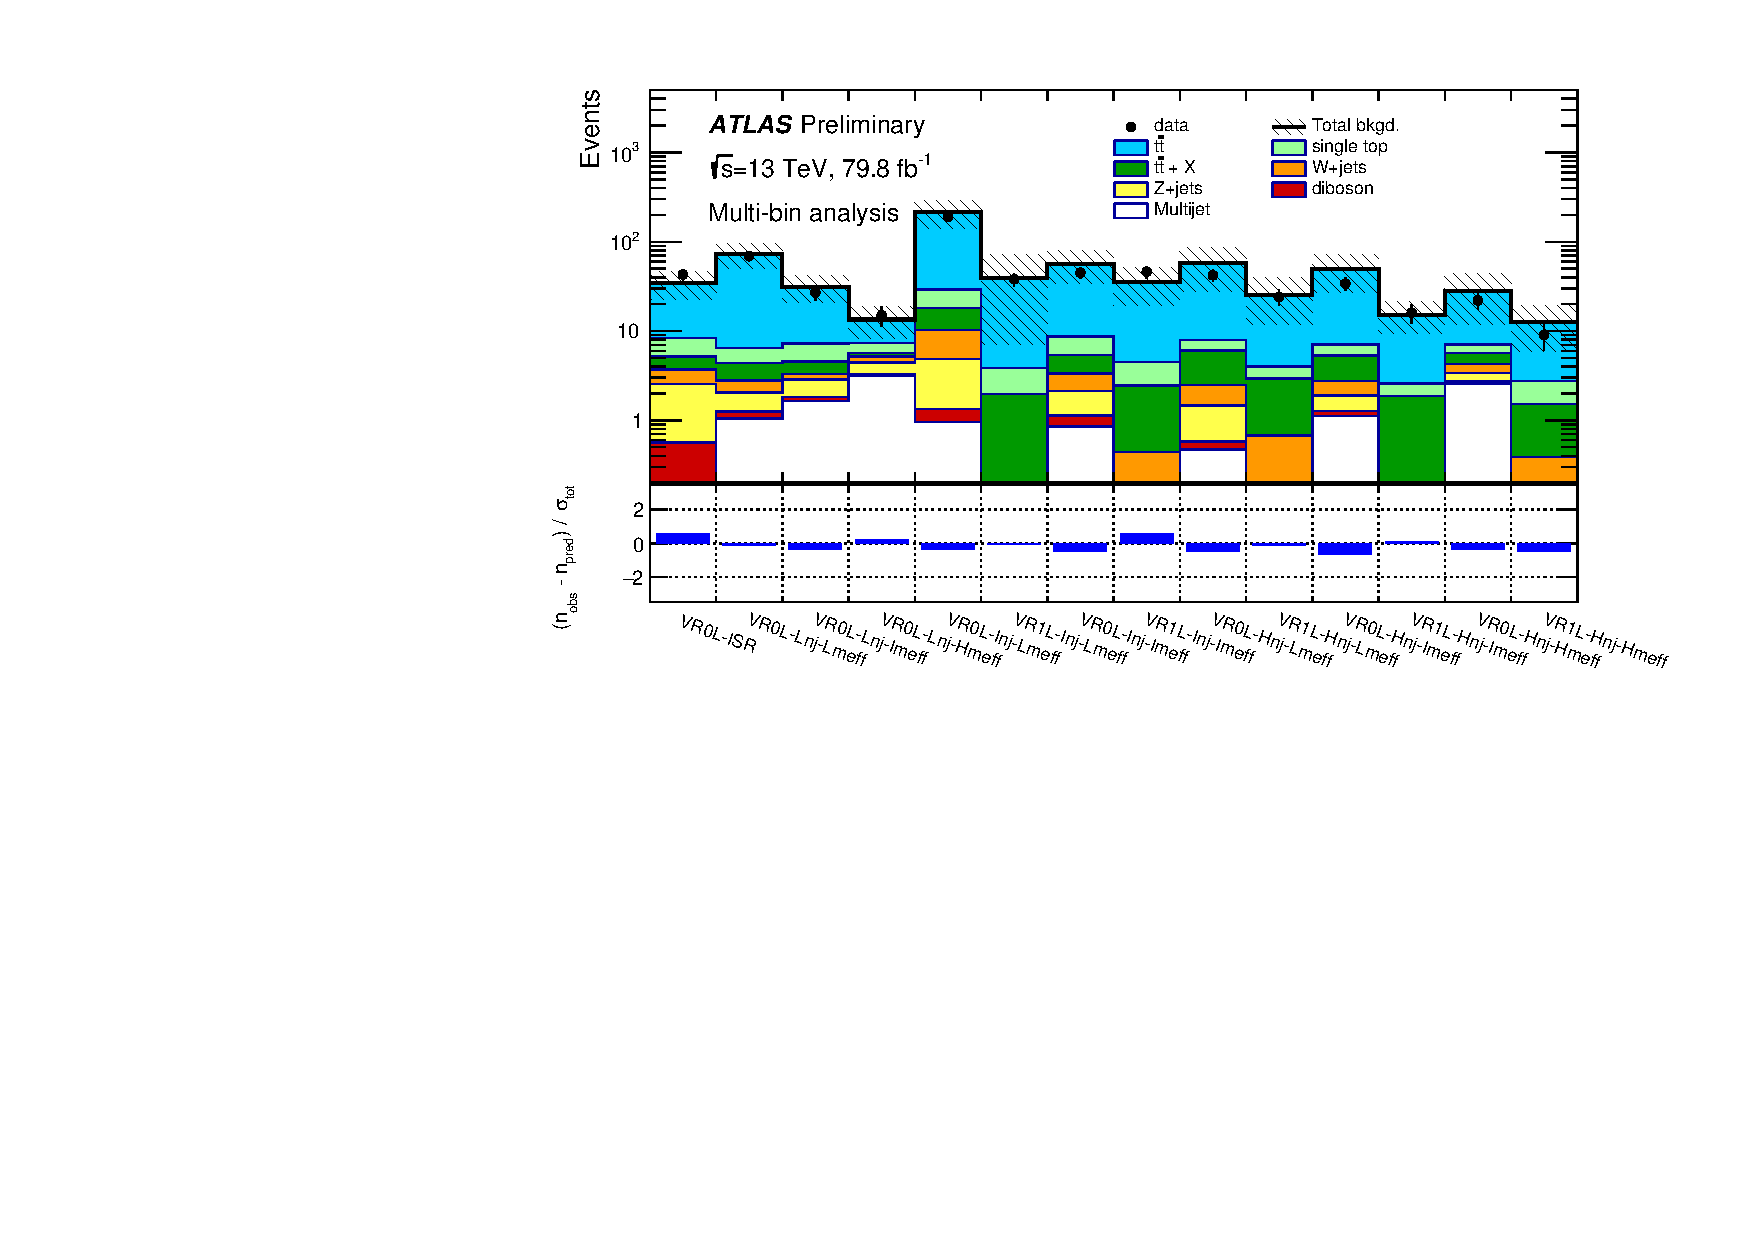
\includegraphics[width=0.9\textwidth]{figures/strong_prod/R21/multibin/histpull_grouping_VR.pdf}\label{fig:pullVR_R21}}\\
%	\subfigure[]{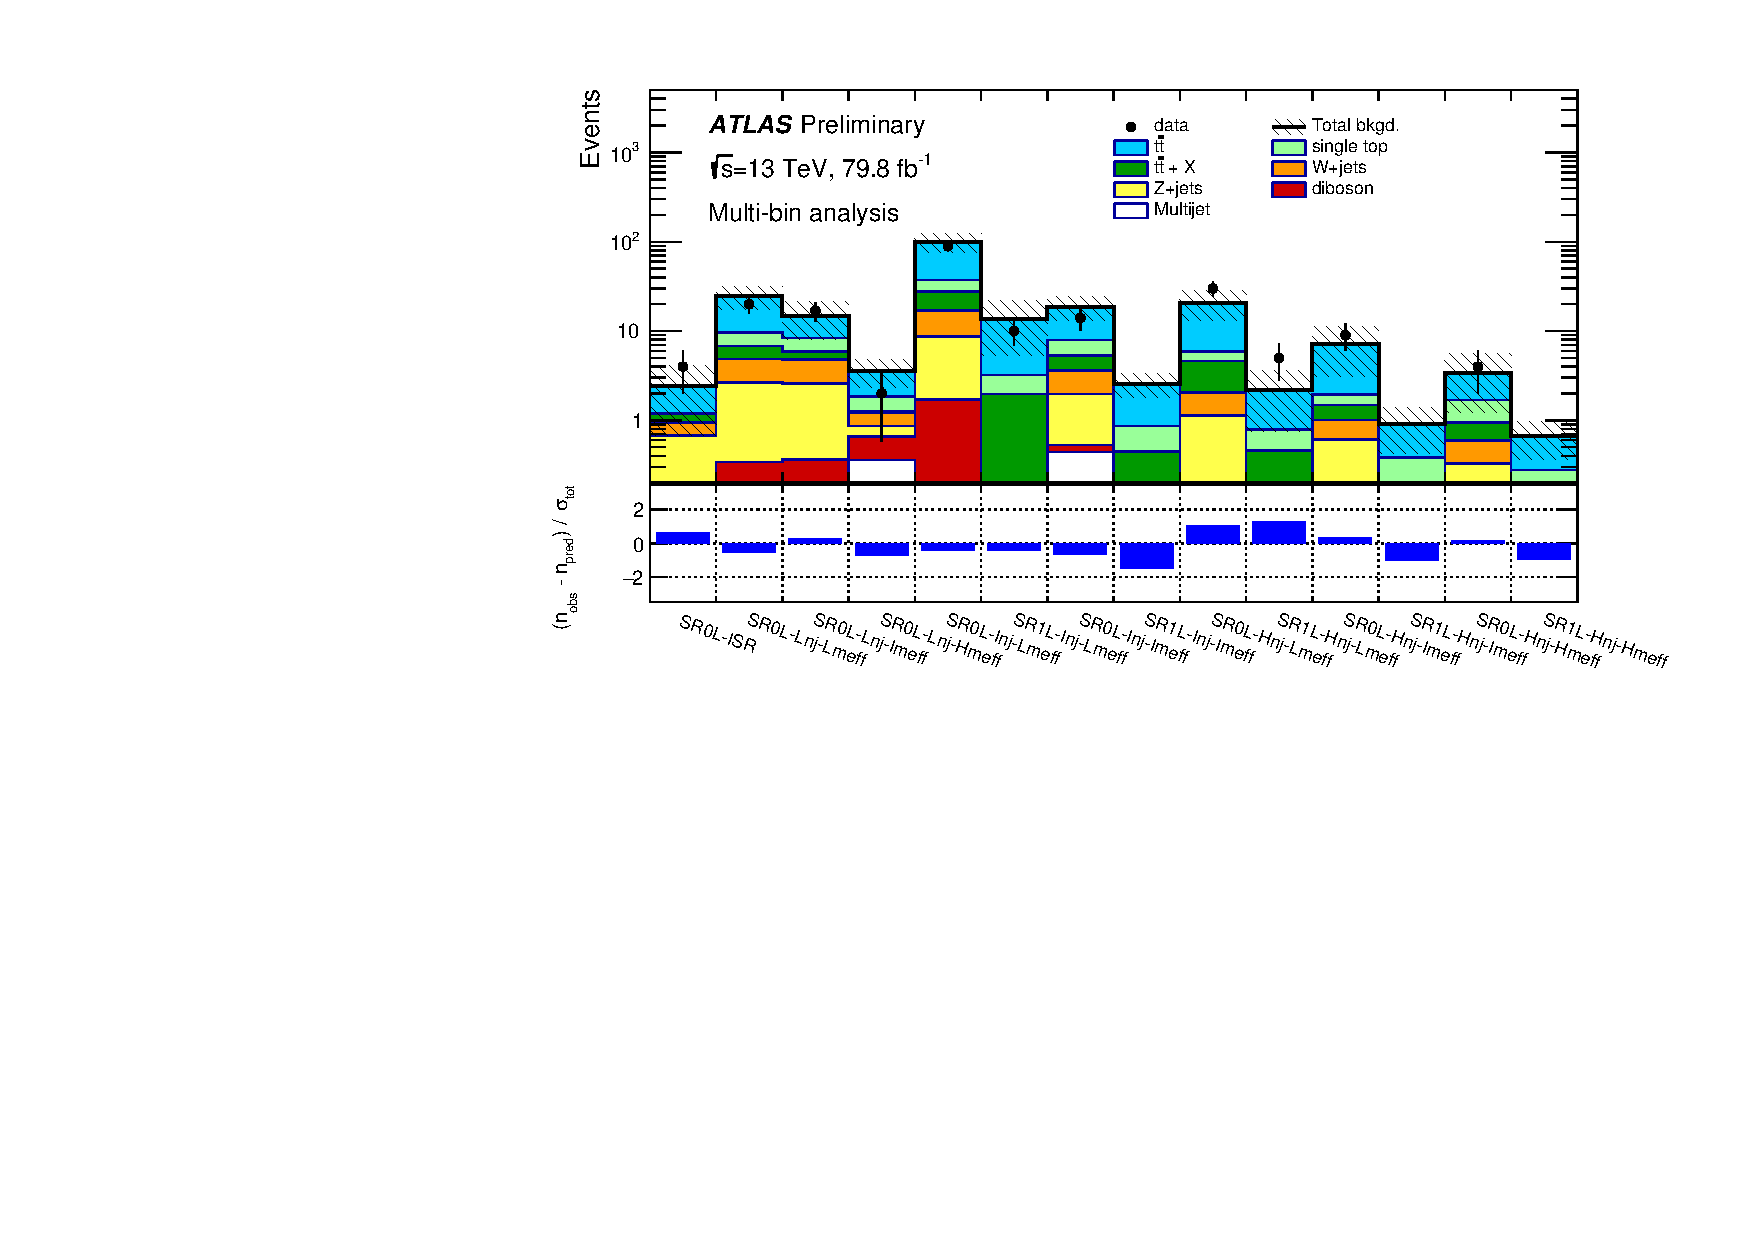
\includegraphics[width=0.9\textwidth]{figures/strong_prod/R21/multibin/histpull_grouping_SR.pdf}\label{fig:pullSR_R21}}\\
%	\caption{Results of the background-only fit extrapolated to the \glspl{vr} for \subref{fig:pullVR_R21}
%	 and to the \glspl{sr} \subref{fig:pullSR_R21} of the multi-bin analyses. 
%	 The data in the  SRs are not included in the fit.  
%	 The upper panel shows the observed number of events and the predicted background 
%	yield. All the experimental and modelling uncertainties as defined in Ref. \cite{ATLAS-CONF-2018-041} are included in the uncertainty band. 
%	The background 
%	category $\ttbar+X$ includes $\ttbar W/Z$, $\ttbar H$ and $\ttbar \ttbar$ events. The lower panel shows the 
%	pull in each region.
%   Figures from Ref. \cite{ATLAS-CONF-2018-041}.	 }  
%	\label{fig:pullR21}
%\end{figure}

\begin{figure}[htbp]
	\centering
	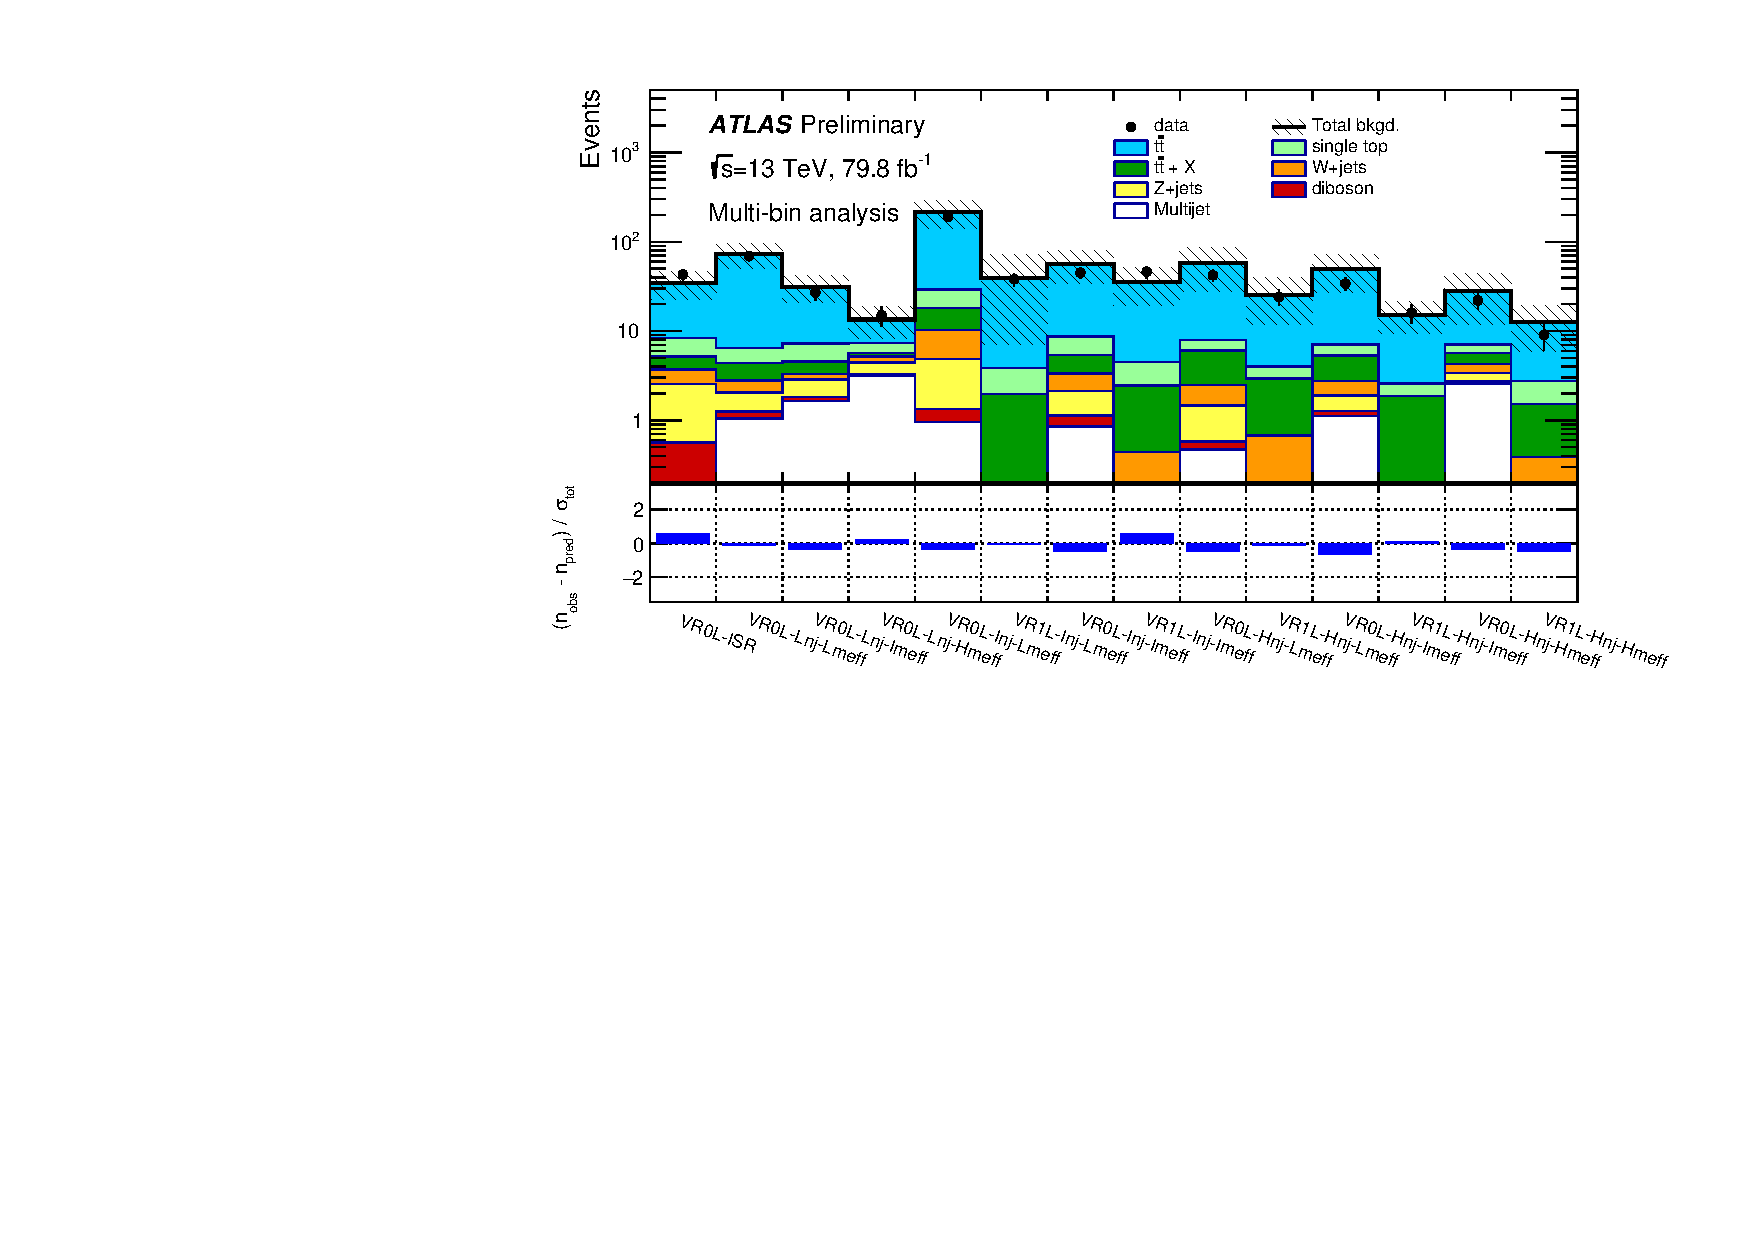
\includegraphics[width=0.9\textwidth]{figures/strong_prod/R21/multibin/histpull_grouping_VR.pdf}\\
	\caption{Results of the background-only fit extrapolated to the \glspl{vr} of the multi-bin analysis. 
	 The data in the  SRs are not included in the fit.  
	 The upper panel shows the observed number of events and the predicted background 
	yield. All the experimental and modelling uncertainties as defined in Ref. \cite{ATLAS-CONF-2018-041} are included in the uncertainty band. 
	The background 
	category $\ttbar+X$ includes $\ttbar W/Z$, $\ttbar H$ and $\ttbar \ttbar$ events. The lower panel shows the 
	pull in each region.
    Figure from Ref. \cite{ATLAS-CONF-2018-041}.	 }  
	\label{fig:pullVR_R21}
\end{figure}

\begin{figure}[htbp]
	\centering
    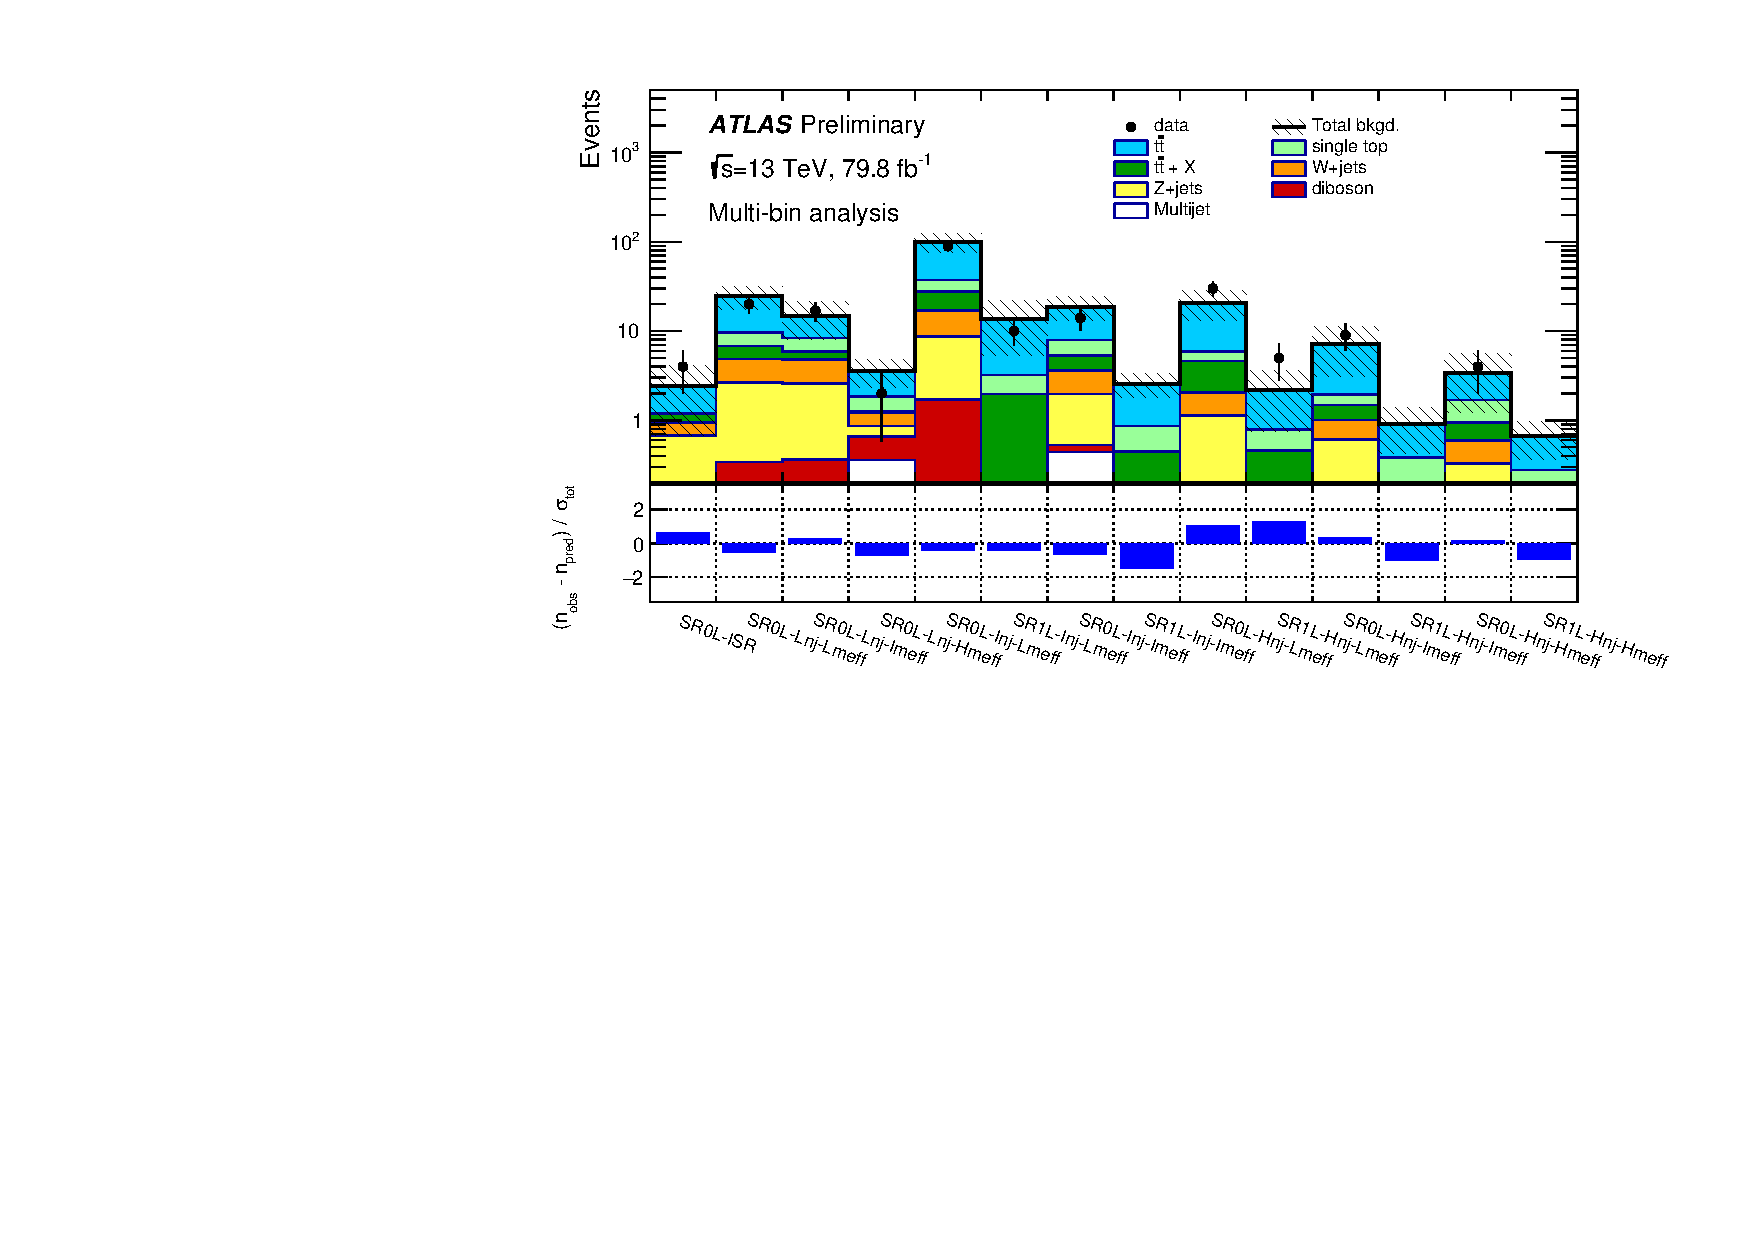
\includegraphics[width=0.9\textwidth]{figures/strong_prod/R21/multibin/histpull_grouping_SR.pdf}
	\caption{Results of the background-only fit extrapolated to the \glspl{sr}  of the multi-bin analysis. 
	 The data in the  SRs are not included in the fit.  
	 The upper panel shows the observed number of events and the predicted background 
	yield. All the experimental and modelling uncertainties as defined in Ref. \cite{ATLAS-CONF-2018-041} are included in the uncertainty band. 
	The background 
	category $\ttbar+X$ includes $\ttbar W/Z$, $\ttbar H$ and $\ttbar \ttbar$ events. The lower panel shows the 
	pull in each region.
    Figure from Ref. \cite{ATLAS-CONF-2018-041}.	 }  
	\label{fig:pullSR_R21}
\end{figure}

\FloatBarrier

\subsection{Interpretation}

In this section, we show the model-dependent limits obtained with the update of the multi-bin analysis to include 79.8 \ifb of data. 
Figures \ref{fig:limits_Gtt_R21} and \ref{fig:limits_Gbb_R21} show the exclusion contour at 95\% \gls{cl} for the Gtt and Gbb 
models respectively; these figures can be compared with the equivalent ones for 36.1 \ifb, Figures \ref{fig:limits_Gtt} and 
\ref{fig:limits_Gbb}. 
The expected sensitivity increases by about 50 and 120 GeV for the Gtt and the Gbb models respectively. 
The difference is larger for the observed limit: 270 for the Gtt model and 280 for the Gbb model. 
This because, while in the 36.1 \ifb analysis the observed limit is weaker than the expected due to 
a few small excesses in the multi-bin analysis, in the 79.8 \ifb 
analysis the observed limits are slightly stronger than the expected in most of the 
m(\gluino)-m(\ninoone) plane. 



\begin{figure}[htbp]
	\centering 
	\subfigure[]{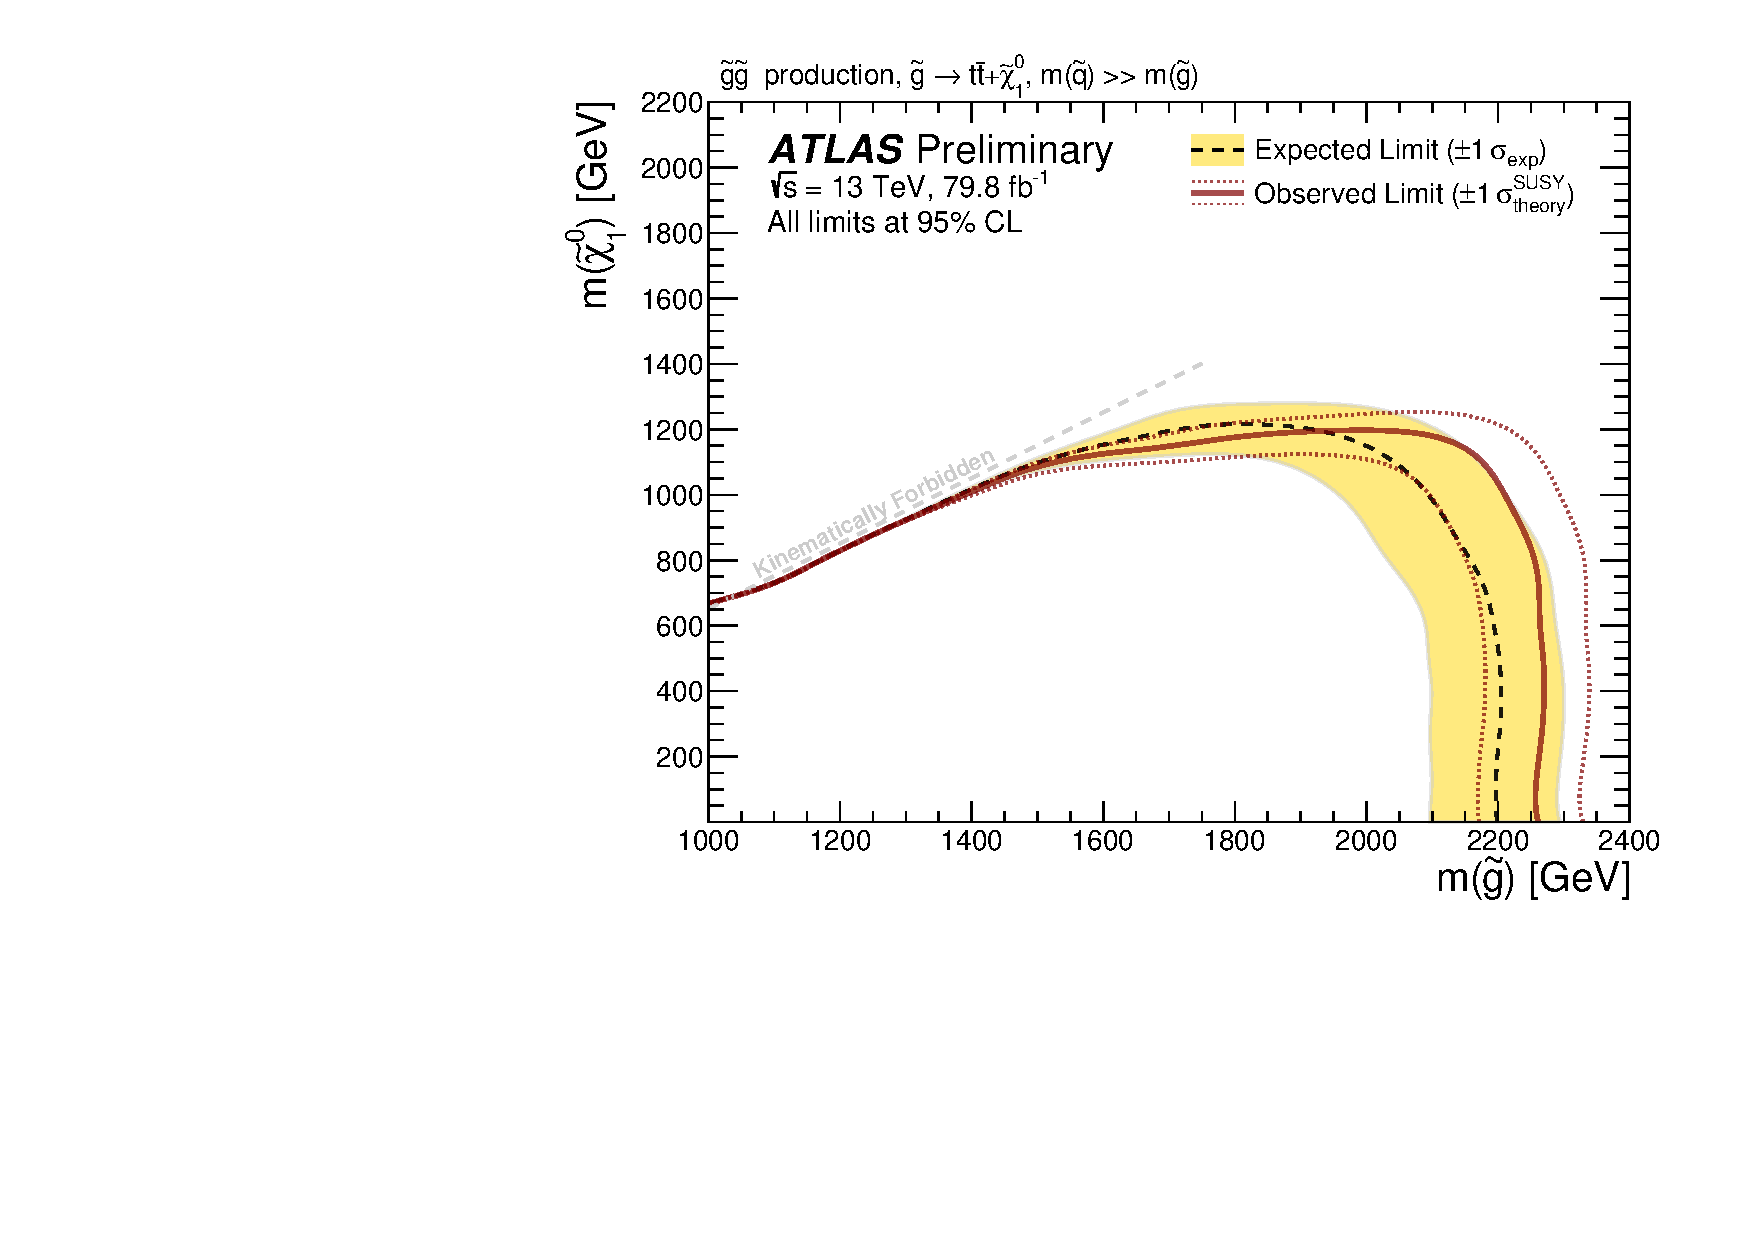
\includegraphics[width=0.49\textwidth]{figures/strong_prod/R21/multibin/3b_tag21_2_27-1_RW_ExpSyst_79800_multibin_excl_Gtt_contour.pdf}\label{fig:limits_Gtt_R21}}
	\subfigure[]{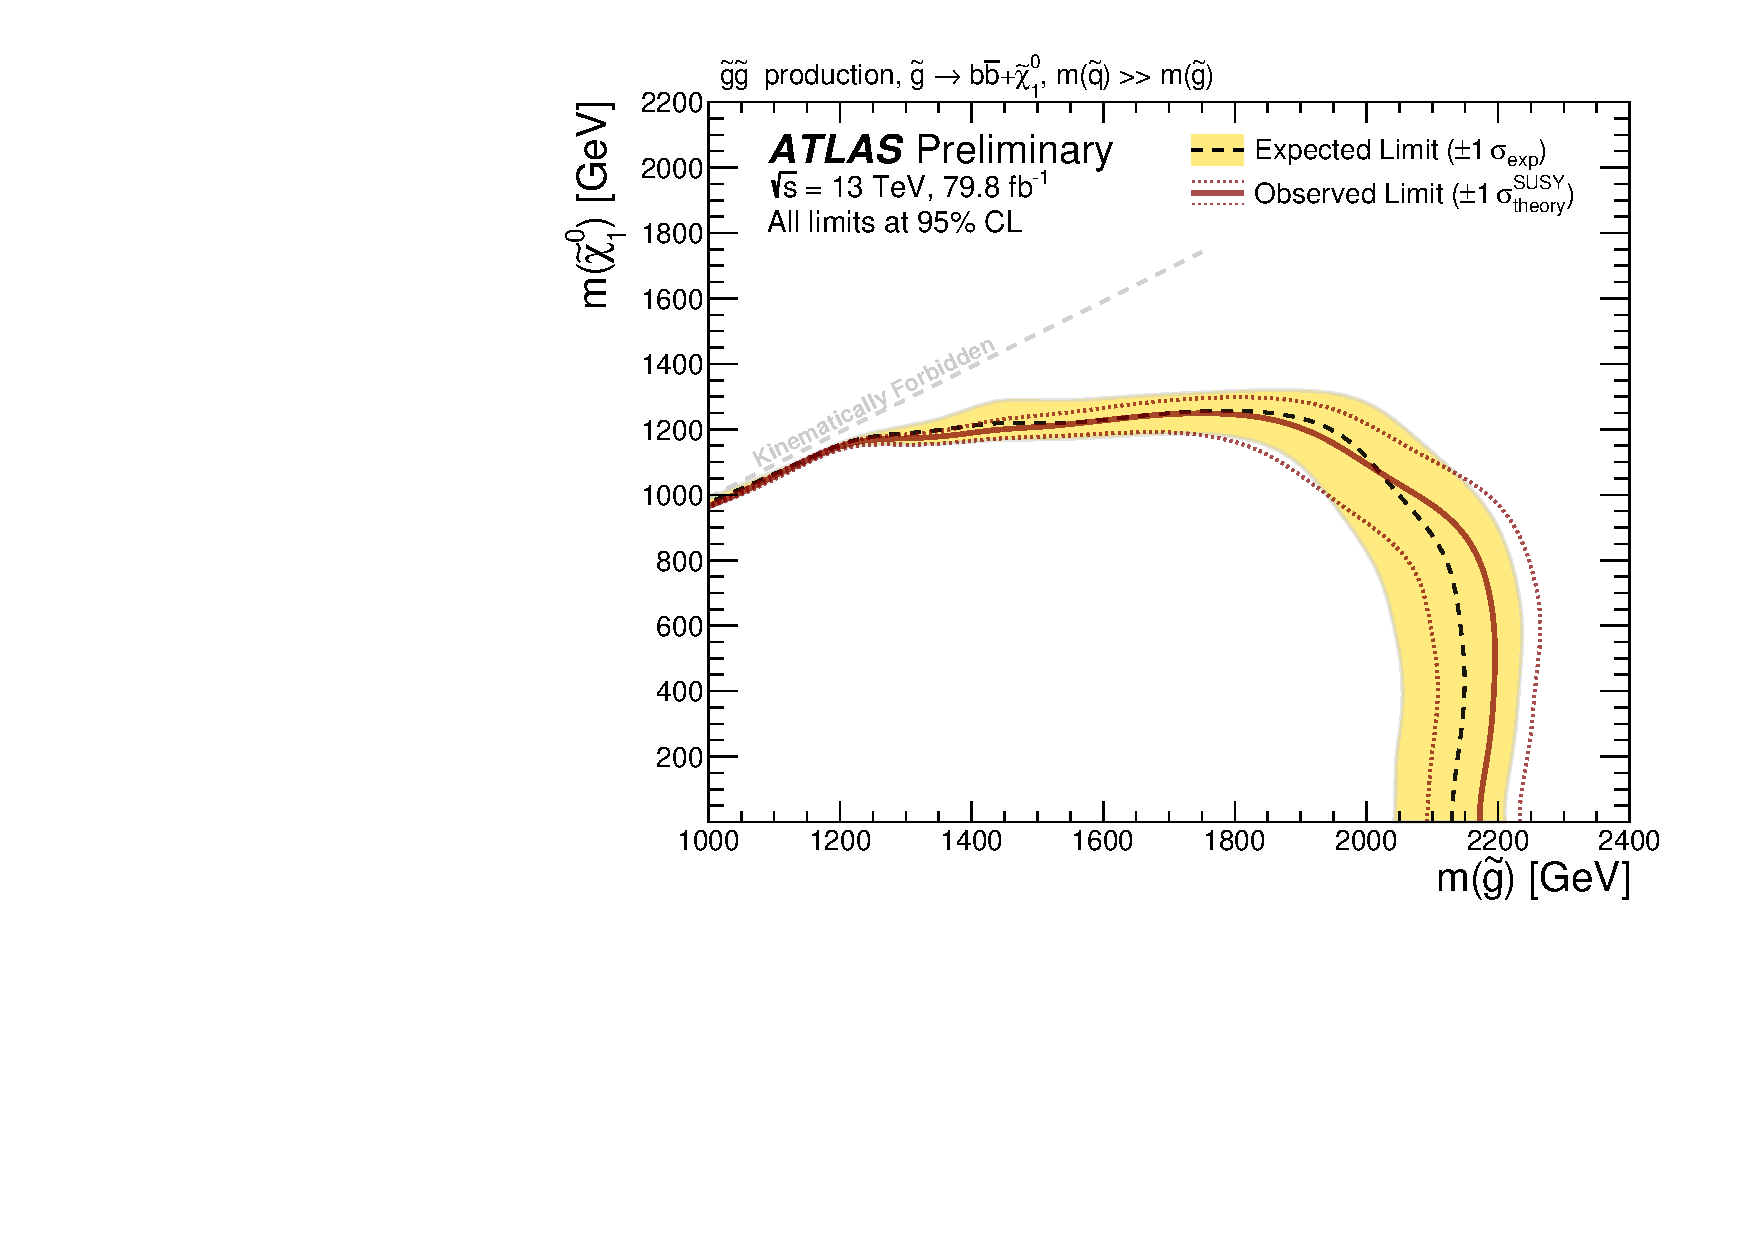
\includegraphics[width=0.49\textwidth]{figures/strong_prod/R21/multibin/3b_tag21_2_27-1_RW_ExpSyst_79800_multibin_excl_Gbb_contour.pdf}\label{fig:limits_Gbb_R21}}
	\caption{Exclusion limits in the $\ninoone$ and $\gluino$ mass plane
  		for the \subref{fig:limits_Gtt_R21} Gtt and  \subref{fig:limits_Gbb_R21} Gbb models obtained
		in the context of the multi-bin analysis. The dashed and solid bold lines
		show the 95\% CL expected and observed limits, respectively. The
  		shaded bands around the expected limits show the
                impact of the
  		experimental and background uncertainties. The dotted
  		lines show the impact on the observed limit of the variation of the
  		nominal signal cross-section by $\pm 1 \sigma$ of its theoretical
  		uncertainty. 
  		Figures from Ref. \cite{ATLAS-CONF-2018-041}.	
      }
	\label{fig:limits_GbbGtt_R21}
\end{figure}

The interpretation with variable \gls{br} of the gluino to $ t \bar{t} \ninoone$, $ b \bar{b} \ninoone$, 
or $t \bar{b} \chinoonem$, and the $\chinoonem$ then decays to $\ninoone$ and soft fermions, but with a different 
presentation choice: for each point in the \gls{br} plane, the highest excluded gluino mass at 95\% \gls{cl}
is shown for a specific neutralino mass. 
Figure~\ref{fig:limits_triangle_1} shows the expected (\ref{fig:limits_triangle_1_exp}) and observed (\ref{fig:limits_triangle_1_obs}) 95\%
\gls{cl} exclusion limits for m(\ninoone) = 1 GeV, while Figures \ref{fig:limits_triangle_600} and \ref{fig:limits_triangle_1000} assume 
m(\ninoone) = 600 GeV and 1 TeV respectively. 
In all the figures, the while lines indicate contours at mass intervals of 50 GeV. 
For a given neutralino mass, the strongest limits for the gluino mass are in the pure-Gtt corner and the weakest ones in the 
pure-Gtb corner for light neutralino mass, while with the increase in neutralino mass the weakest-exclusion point 
moves to points with higher \gls{br} to $ b \bar{b} \ninoone$.


\begin{figure}[htbp]
  \centering 
  \subfigure[]{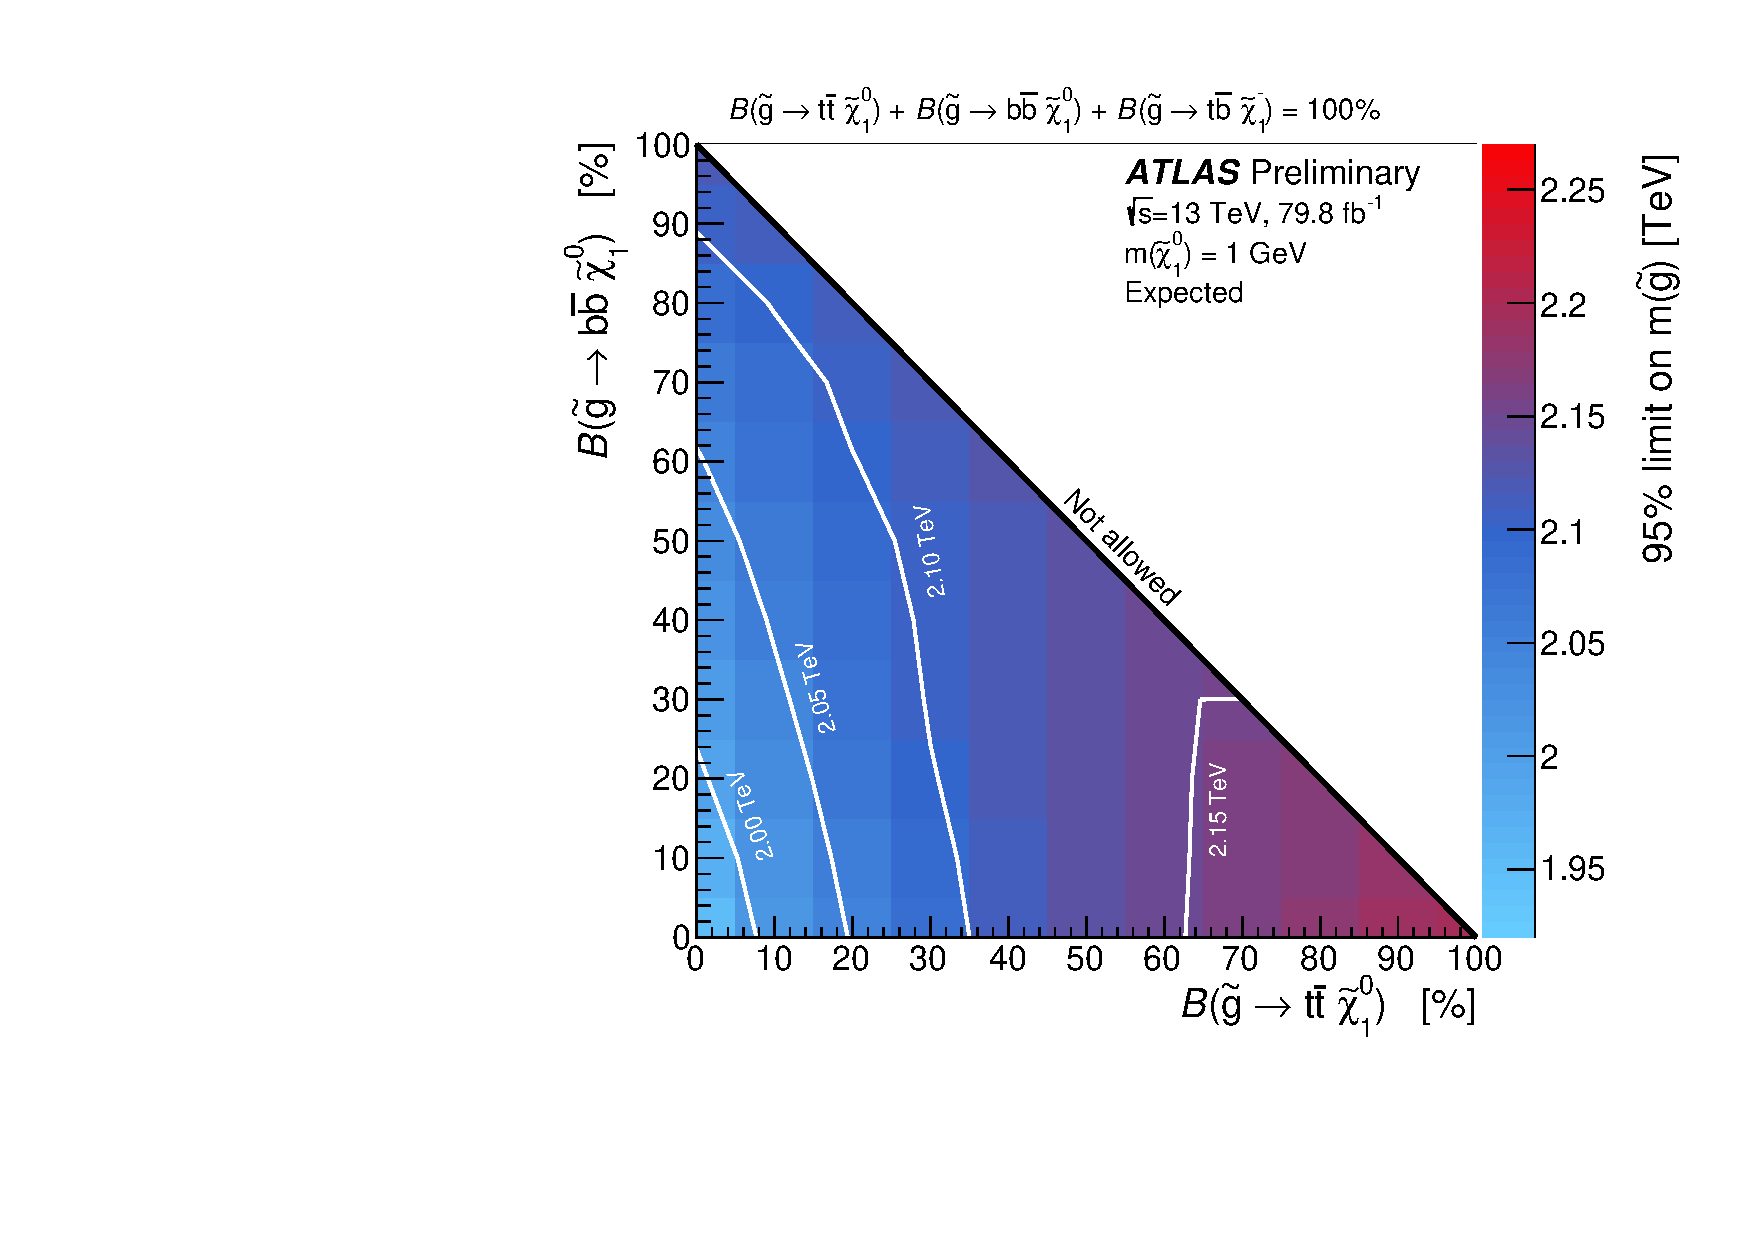
\includegraphics[width=0.49\textwidth]{figures/strong_prod/R21/multibin/triangle_5000_1_expected}\label{fig:limits_triangle_1_exp}}
  \subfigure[]{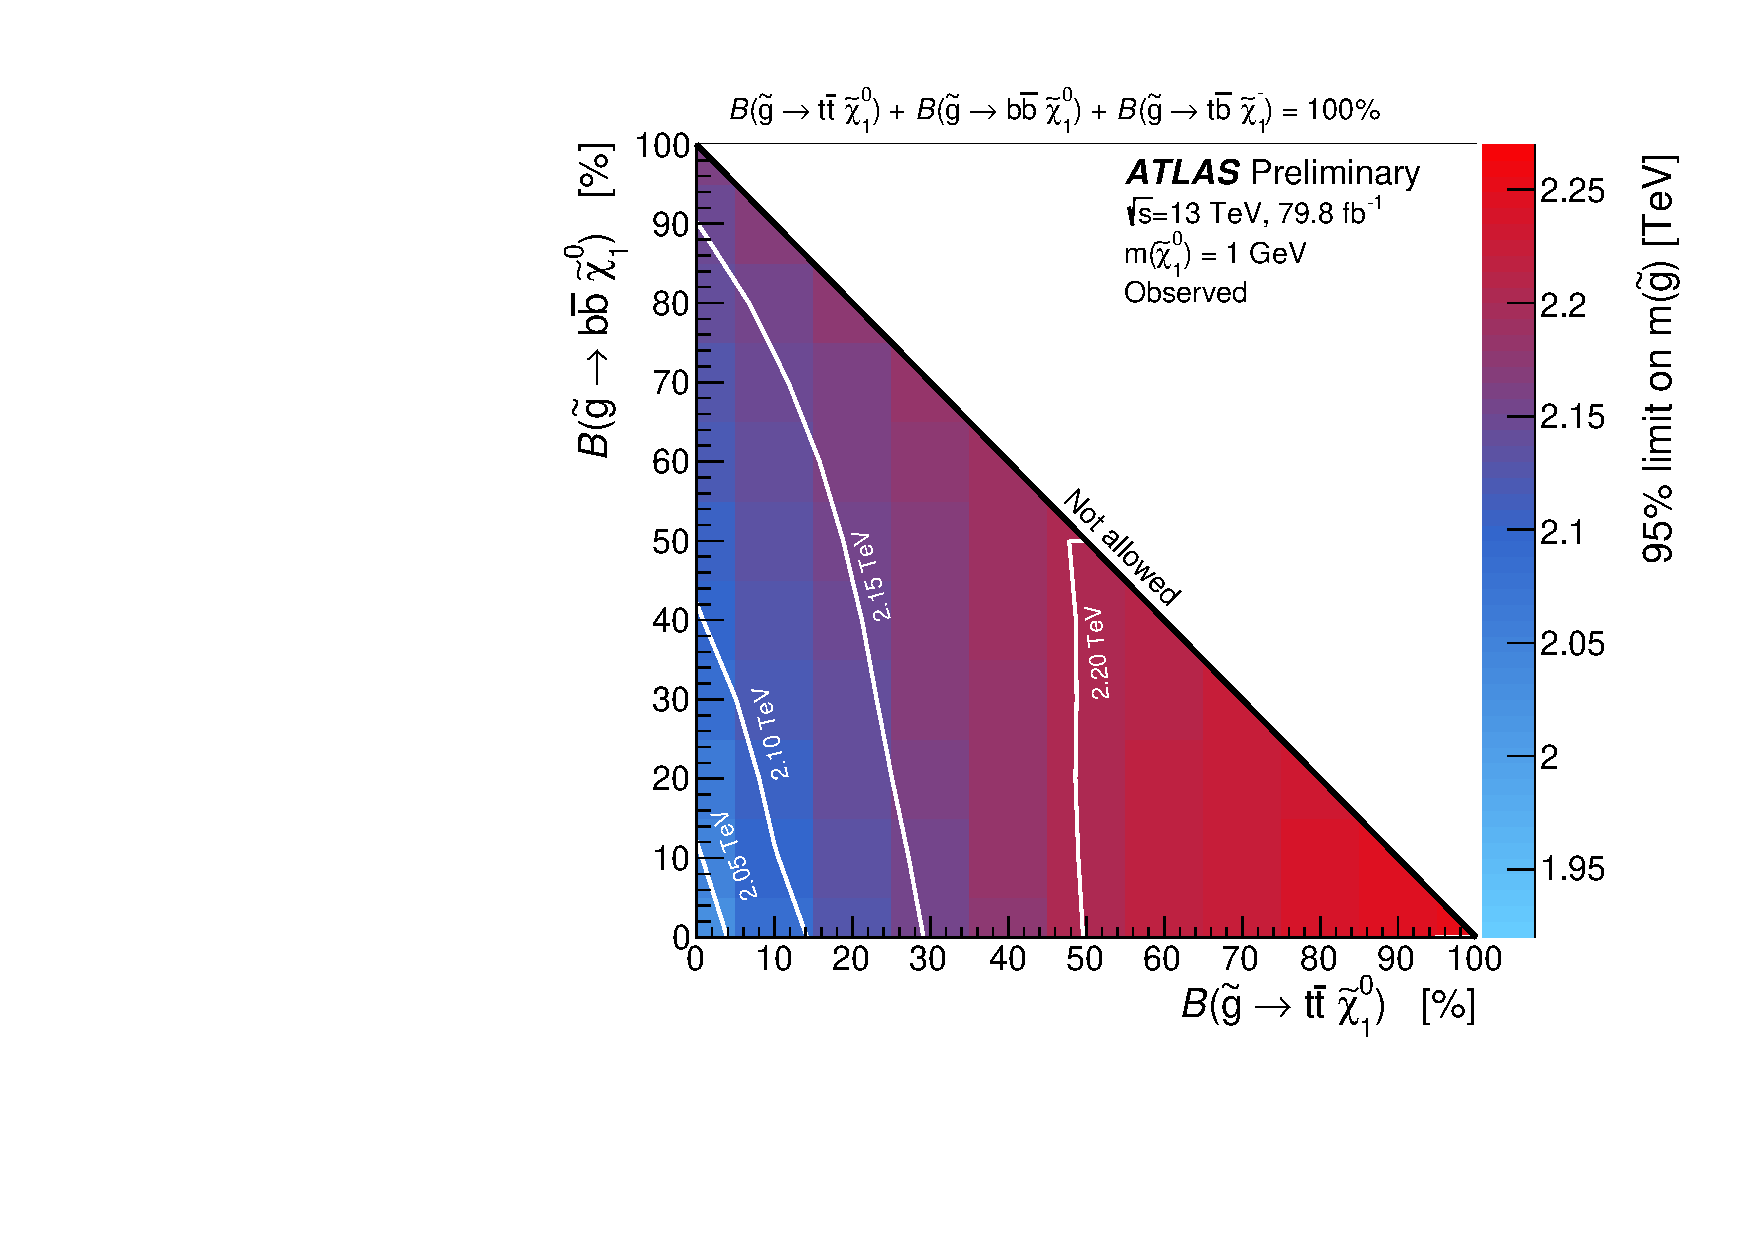
\includegraphics[width=0.49\textwidth]{figures/strong_prod/R21/multibin/triangle_5000_1_observed}\label{fig:limits_triangle_1_obs}}
  \caption{The expected \subref{fig:limits_triangle_1_exp} and observed \subref{fig:limits_triangle_1_obs} 95\%~CL exclusion limits on the gluino mass as a function of the gluino branching ratio to Gbb (vertical) and Gtt (horizontal) models. Gluinos not decaying to either the Gtt or Gbb mode are assumed to decay via Gtb instead. In this figure \mchi is fixed to 1 GeV. The $z$-axis indicates the maximum excluded gluino mass for each point in the branching ratio space. The white lines indicate contours at mass intervals of 50 GeV. The exclusion limits were derived using the multibin analysis.
  Figures from Ref. \cite{ATLAS-CONF-2018-041}.}
  \label{fig:limits_triangle_1}
\end{figure}

\begin{figure}[htbp]
  \centering 
  \subfigure[]{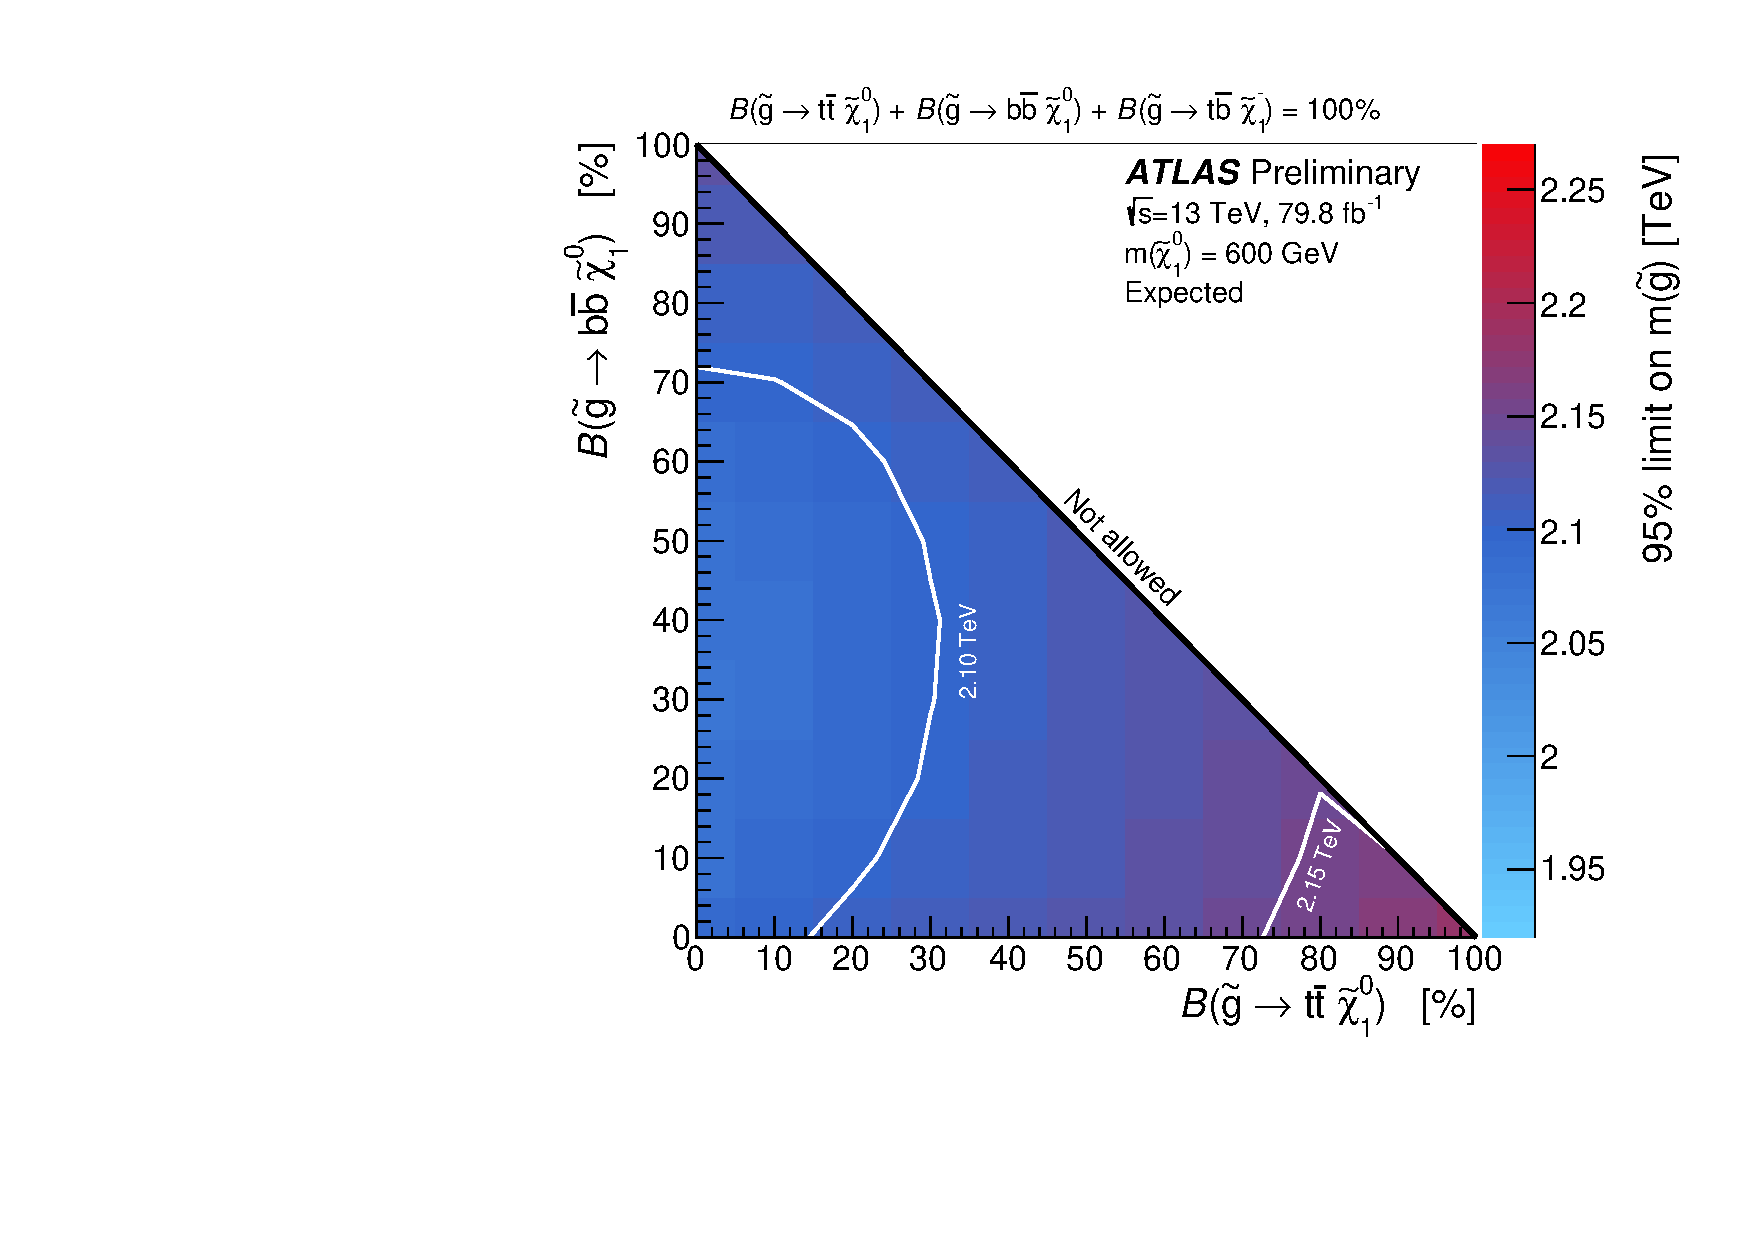
\includegraphics[width=0.49\textwidth]{figures/strong_prod/R21/multibin/triangle_5000_600_expected}\label{fig:limits_triangle_600_exp}}
  \subfigure[]{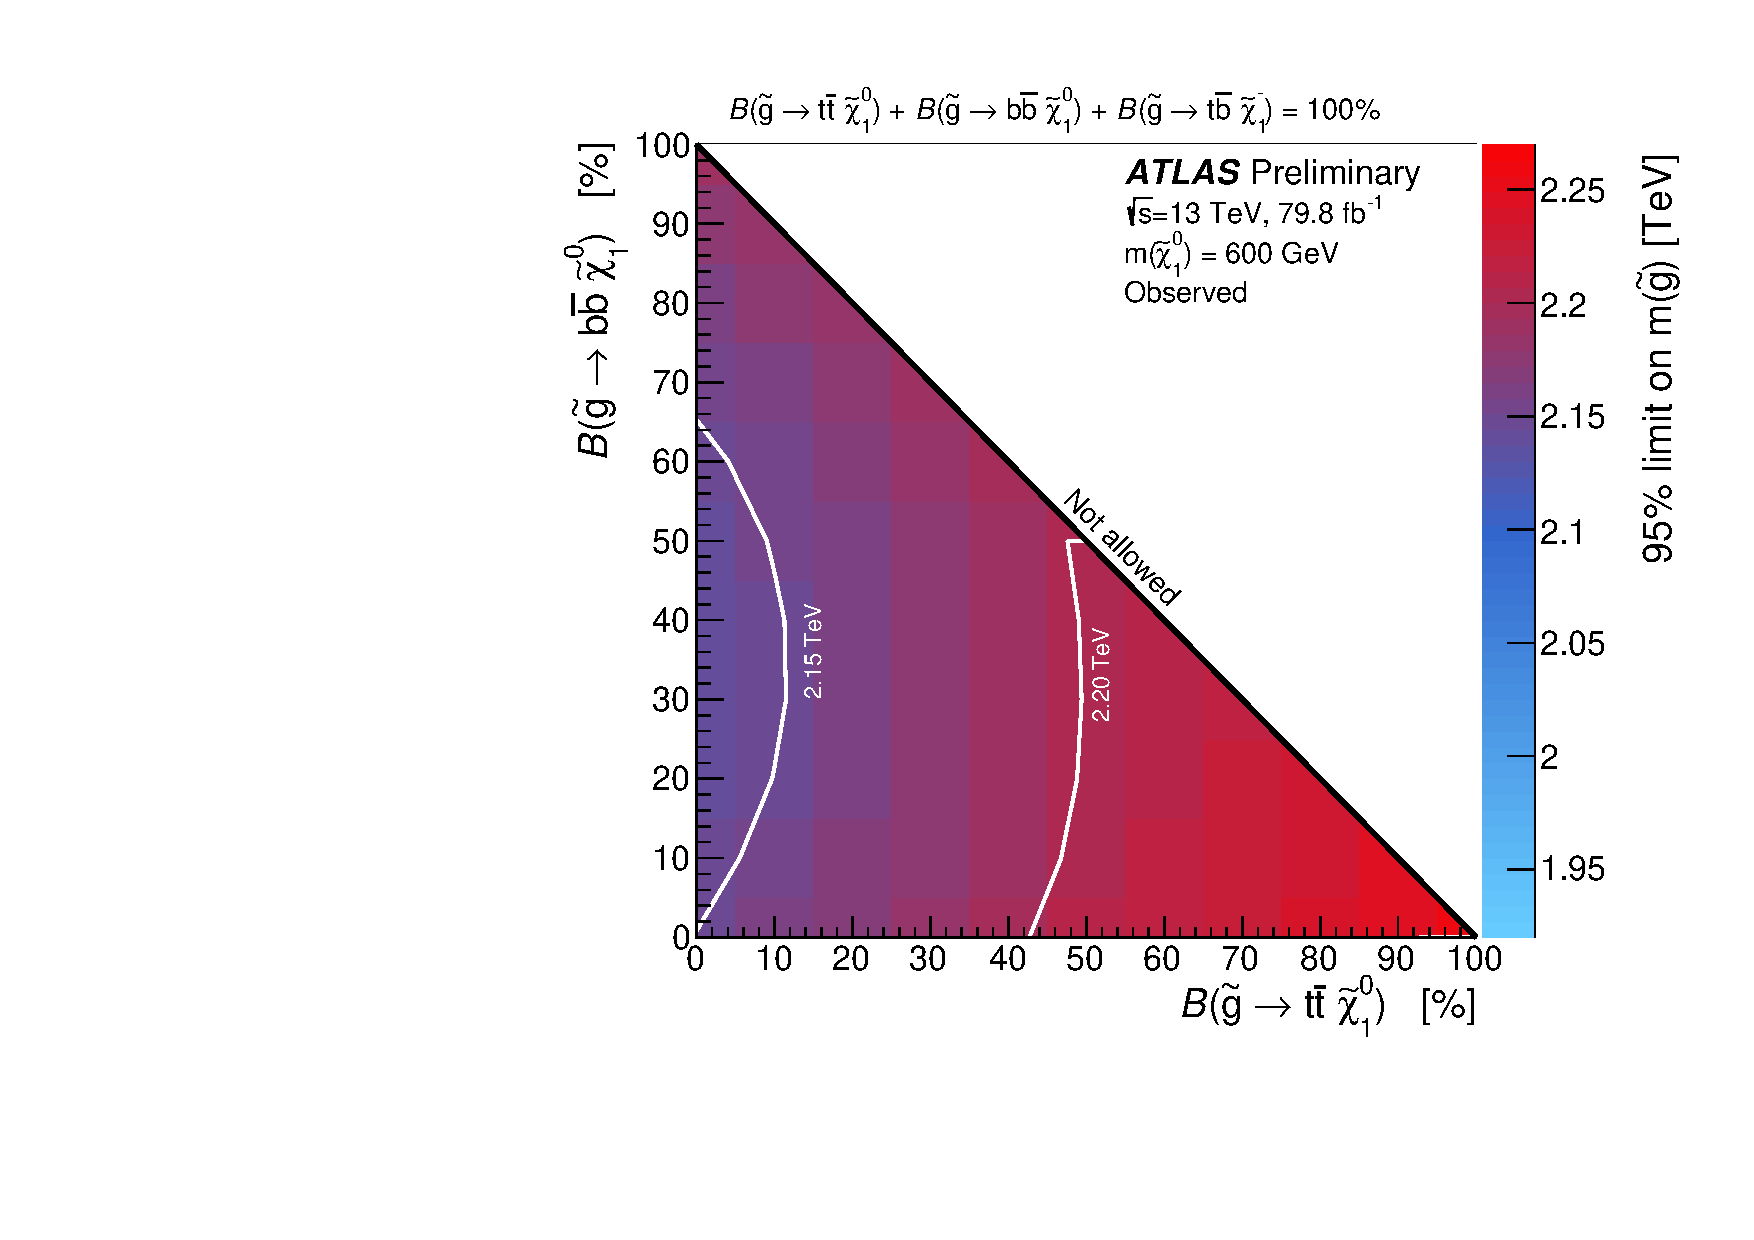
\includegraphics[width=0.49\textwidth]{figures/strong_prod/R21/multibin/triangle_5000_600_observed}\label{fig:limits_triangle_600_obs}}
  \caption{The expected \subref{fig:limits_triangle_1_exp} and observed \subref{fig:limits_triangle_1_obs} 95\%~CL exclusion limits on the gluino mass as a function of the gluino branching ratio to Gbb (vertical) and Gtt (horizontal) models. Gluinos not decaying to either the Gtt or Gbb mode are assumed to decay via Gtb instead. In this figure \mchi is fixed to 600 GeV. The $z$-axis indicates the maximum excluded gluino mass for each point in the branching ratio space. The white lines indicate contours at mass intervals of 50 GeV. The exclusion limits were derived using the multibin analysis.
  Figures from Ref. \cite{ATLAS-CONF-2018-041}.
      }
  \label{fig:limits_triangle_600}
\end{figure}

\begin{figure}[htbp]
  \centering 
  \subfigure[]{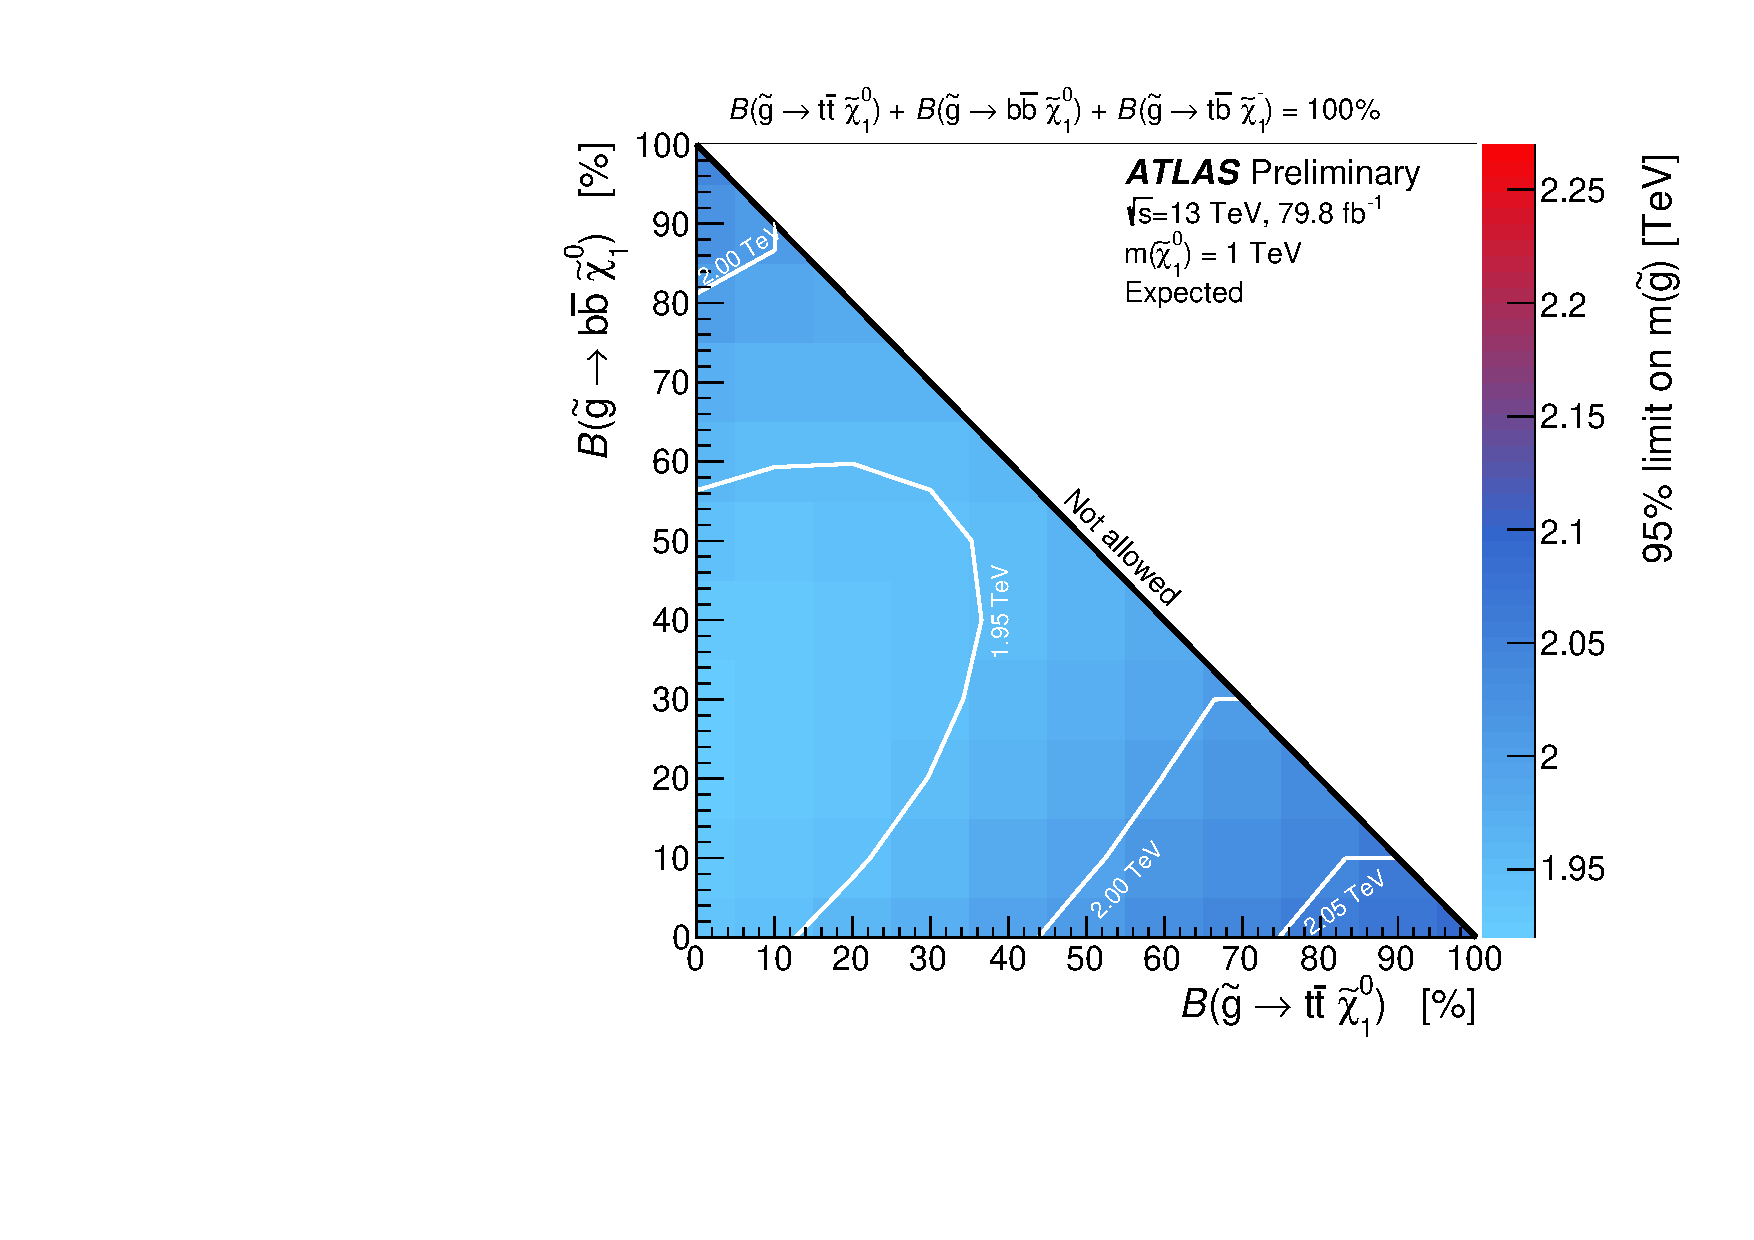
\includegraphics[width=0.49\textwidth]{figures/strong_prod/R21/multibin/triangle_5000_1000_expected}\label{fig:limits_triangle_1000_exp}}
  \subfigure[]{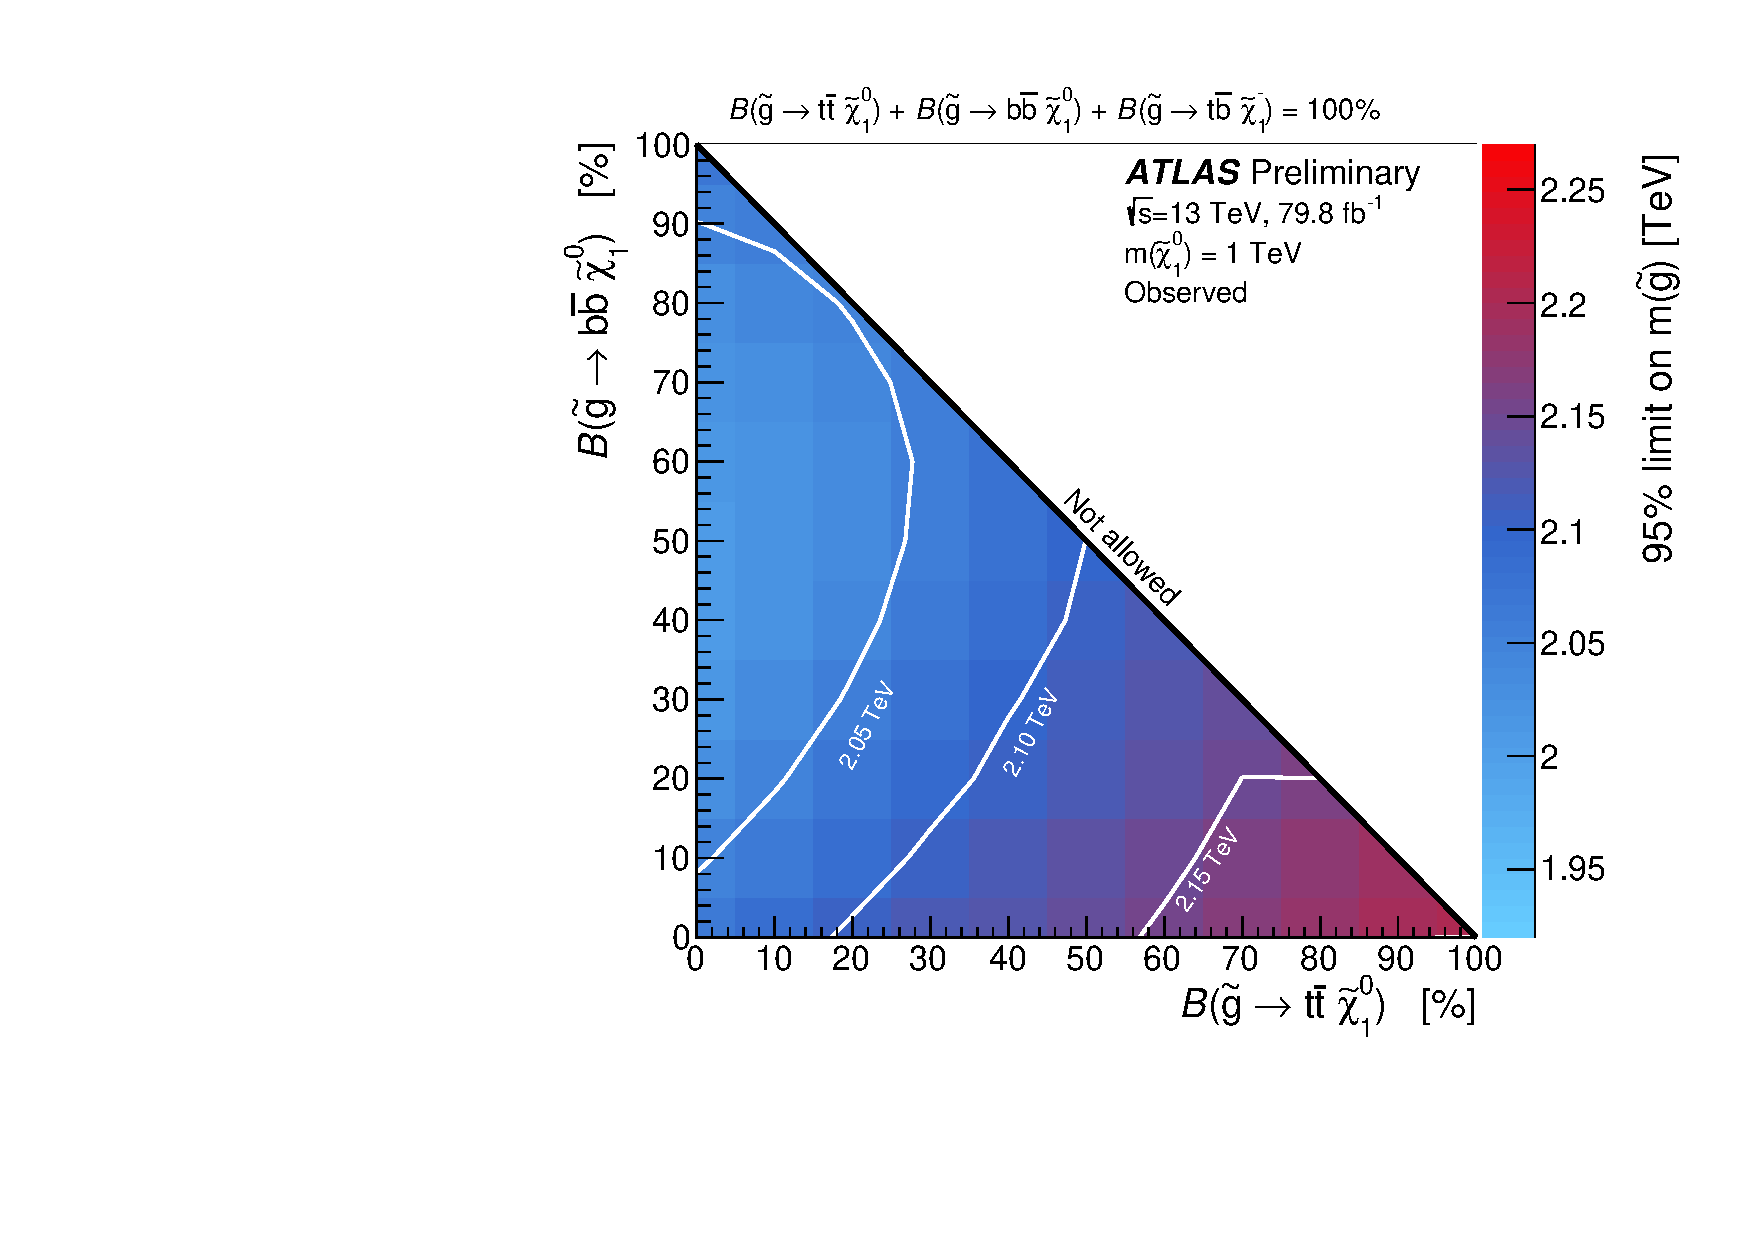
\includegraphics[width=0.49\textwidth]{figures/strong_prod/R21/multibin/triangle_5000_1000_observed}\label{fig:limits_triangle_1000_obs}}
  \caption{The expected \subref{fig:limits_triangle_1_exp} and observed \subref{fig:limits_triangle_1_obs} 95\%~CL exclusion limits on the gluino mass as a function of the gluino branching ratio to Gbb (vertical) and Gtt (horizontal) models. Gluinos not decaying to either the Gtt or Gbb mode are assumed to decay via Gtb instead. In this figure \mchi is fixed to 1000 GeV. The $z$-axis indicates the maximum excluded gluino mass for each point in the branching ratio space. The white lines indicate contours at mass intervals of 50 GeV. The exclusion limits were derived using the multibin analysis.
  Figures from Ref. \cite{ATLAS-CONF-2018-041}.}
  \label{fig:limits_triangle_1000}
\end{figure}


Two additional interpretations have been included in this version of the analysis, to test the dependence of the limits on the 
assumption on m($\tilde{t}$) for the Gtt model and on m($\tilde{t}$), m($\tilde{b}$) and m(\chinoonepm) for the model with mixed \glspl{br}.
In the case of the Gtt model, the nominal exclusion limit is provided assuming an off-shell stop: m($\tilde{t}$) is set to 5 TeV.
Figure \ref{fig:limits_GttOnshell} shows the expected and observed 95\% cross section upper limit for a signal model with 
m(\gluino) = 2.1 TeV and m(\ninoone) = 600 GeV as a function of the stop mass; the thin blue lines 
show the limit in the case of off-shell stop. 
The range chosen for  m($\tilde{t}$) allows an on-shell decay for both 
$\gluino \to \tilde{t}t$ and $\tilde{t} \to t \ninoone$. 
We can see that while for intermediate values of m($\tilde{t}$) the sensitivity is similar (and for some masses even better) 
than the off-shell case, when m($\tilde{t}$) is close to the kinematic boundary of 
m(\ninoone)+m($t$) and m(\gluino)-m($t$) the sensitivity degrades. 
This is because when m($\tilde{t}$) approaches m(\ninoone)+m($t$), the top quark originating from the $\tilde{t}$ decay 
has low momentum; instead, when m($\tilde{t}$) approaches m(\gluino)-m($t$), is the top quark produced in the \gluino 
decay that has less energy than in the off-shell case, limiting the sensitivity of the analysis. 


\begin{figure}
  \centering
  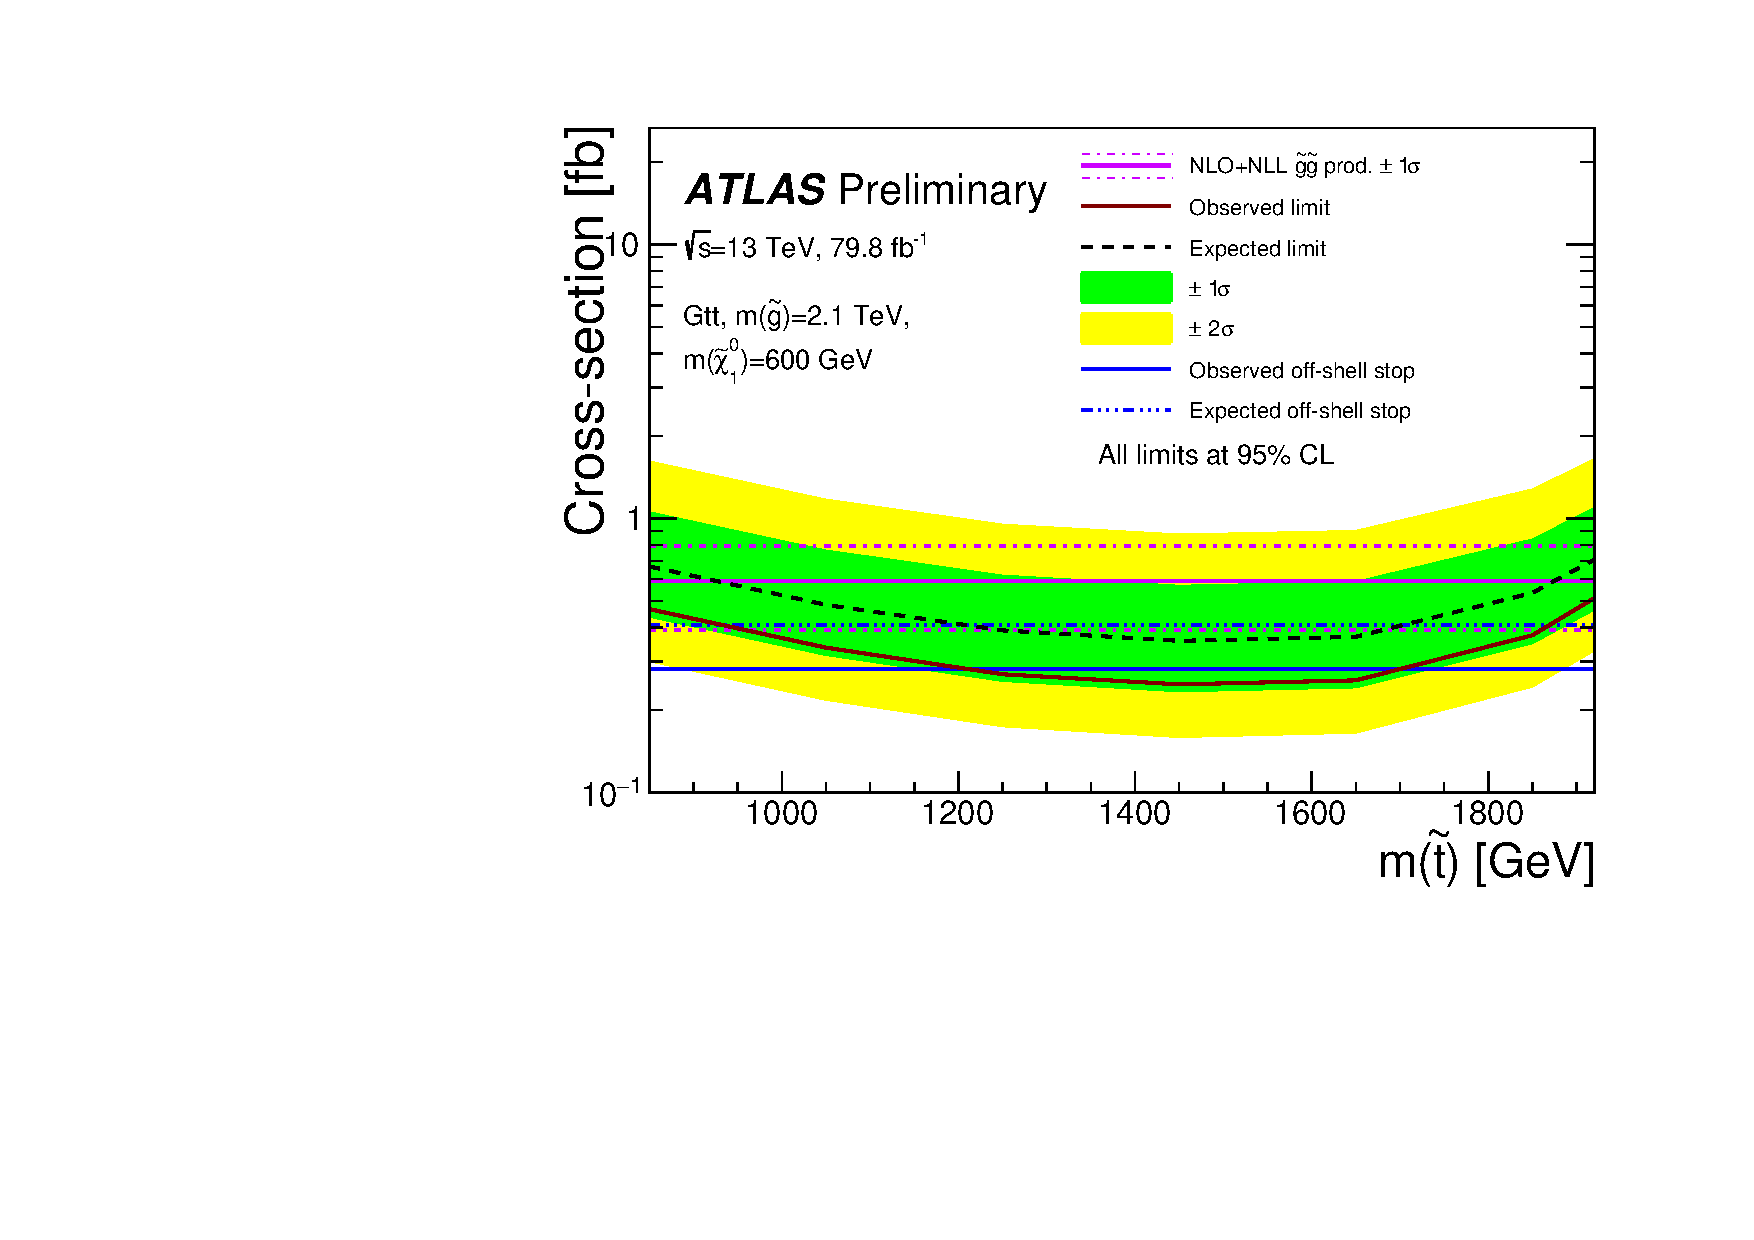
\includegraphics[width=0.75\textwidth]{figures/strong_prod/R21/multibin/Gtt_2100_600_onshell}
  \caption{Exclusion limits as a function of m($\tilde{t}$), in the Gtt model but with an on-shell stop, in the context of the multi-bin analysis. The $\tilde{g}$ and \ninoone masses are fixed to 2.1 TeV and 600 GeV respectively. The dashed and solid bold lines
    show the 95\% CL expected and observed limits, respectively. The solid red line indicates the theoretical cross-section for a 2.1 TeV gluino. The thin blue lines indicate the expected (dashed) and observed (solid) limits for the case of the off-shell stop, where m($\tilde{t}$) = 5 TeV.
    Figures from Ref. \cite{ATLAS-CONF-2018-041}.}
  \label{fig:limits_GttOnshell}
\end{figure}

The second additional interpretation is presented in 
Figure~\ref{fig:limits_GtbOnshell}, showing the expected and observed the 95\%~CL cross-section upper limit for the mixed-\gls{br}
 model with on-shell stop, sbottom and $\chinoonepm$, as a function of the stop mass.
The signal model considered had m(\gluino) = 2.1 TeV, m(\ninoone) = 600 GeV, m($\tilde{b}$) = m($\tilde{t}$), 
and the $\chinoonepm$ mass fixed to 1.2 TeV and 
180 GeV lower than the stop mass in Figures \ref{fig:limits_GtbOnshell_1200}  and \ref{fig:limits_GtbOnshell_diff180} respectively.
In the case of fixed m($\chinoonepm$), the limit does not display a strong dependence on 
In the range considered for the masses of stop and sbottom, the cross-section limit on m($\tilde{t}$) and m($\tilde{b}$) in 
the case of  $\chinoonepm$ mass fixed to 1.2 TeV. 
Instead when m($\chinoonepm$) increases with m($\tilde{t}$),
we can see that the limit weakens at high m($\tilde{t}$).

\begin{figure}
  \centering
  \subfigure[]{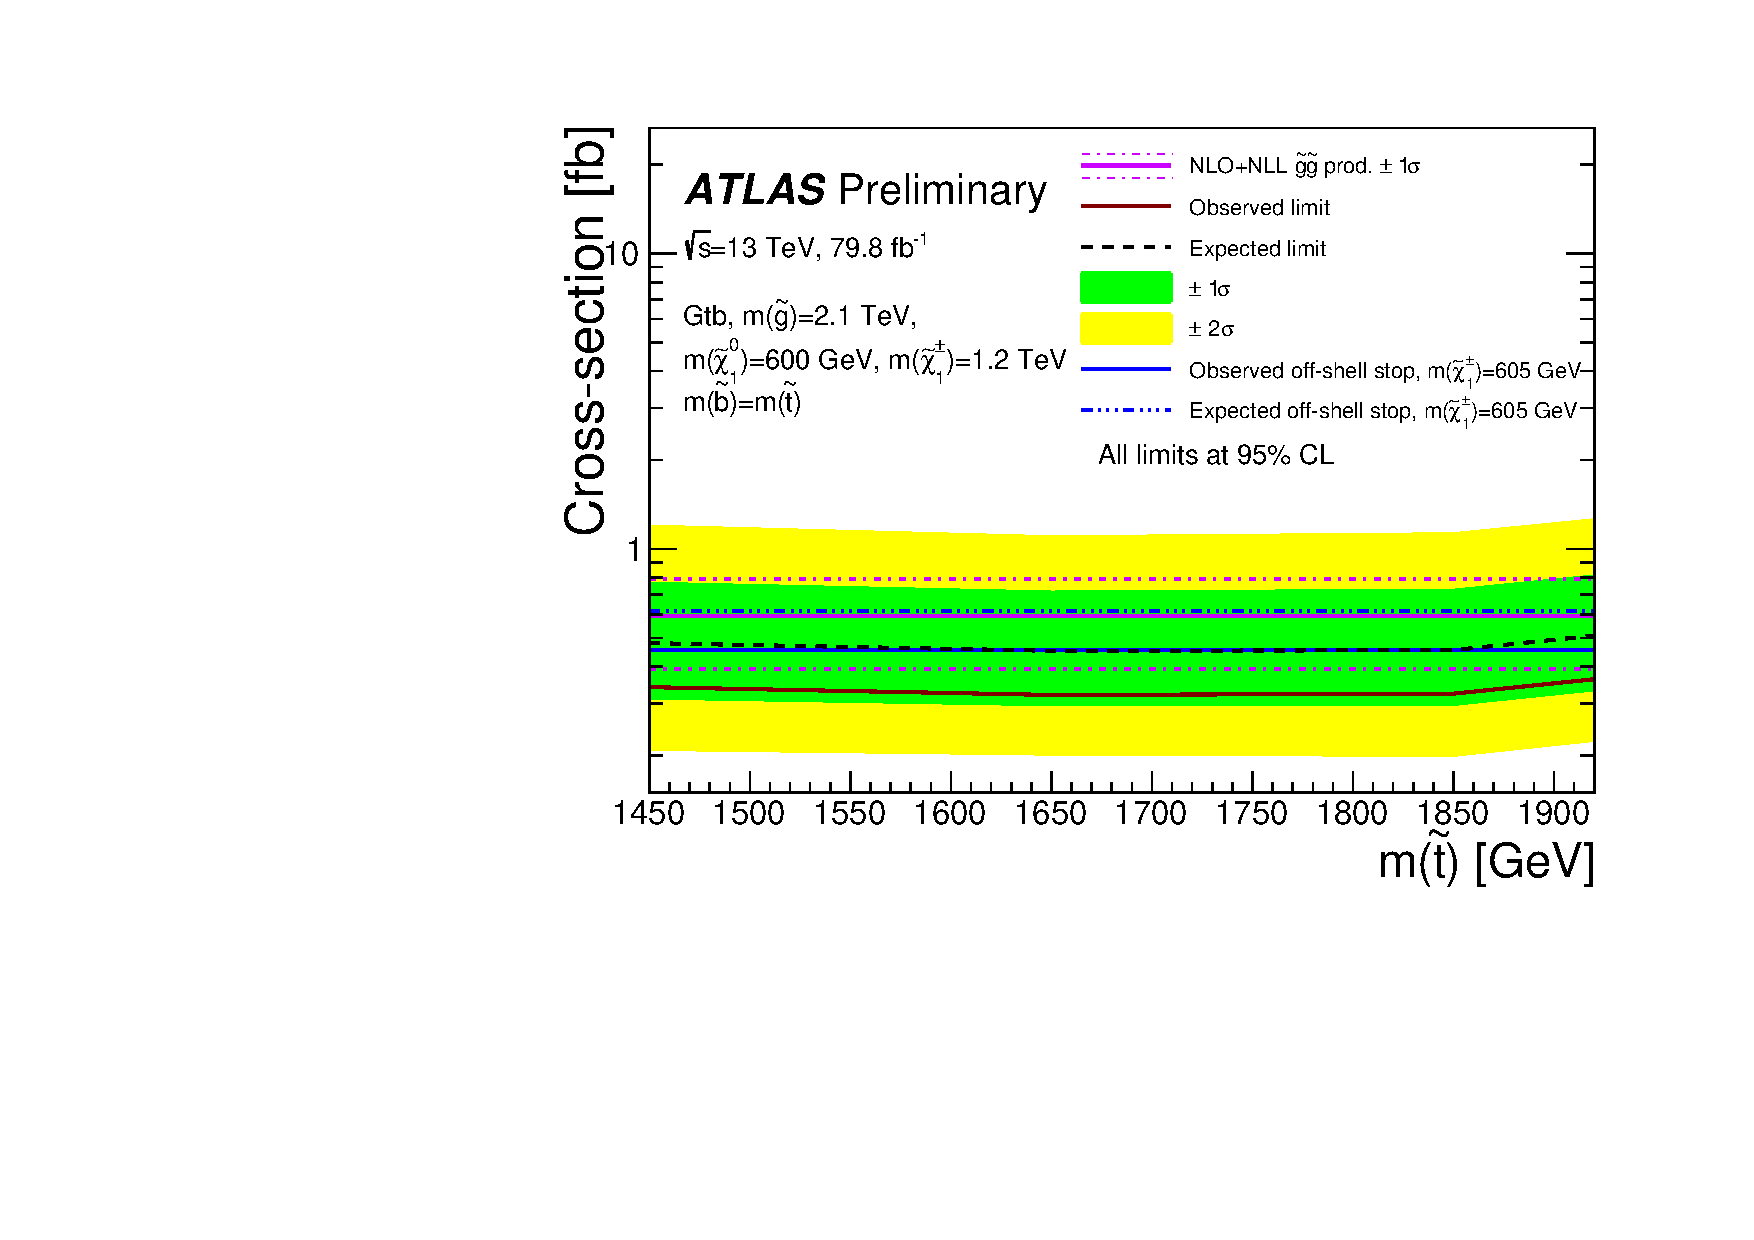
\includegraphics[width=0.75\textwidth]{figures/strong_prod/R21/multibin/Gtb_2100_1200_600_onshell}\label{fig:limits_GtbOnshell_1200}}
  \subfigure[]{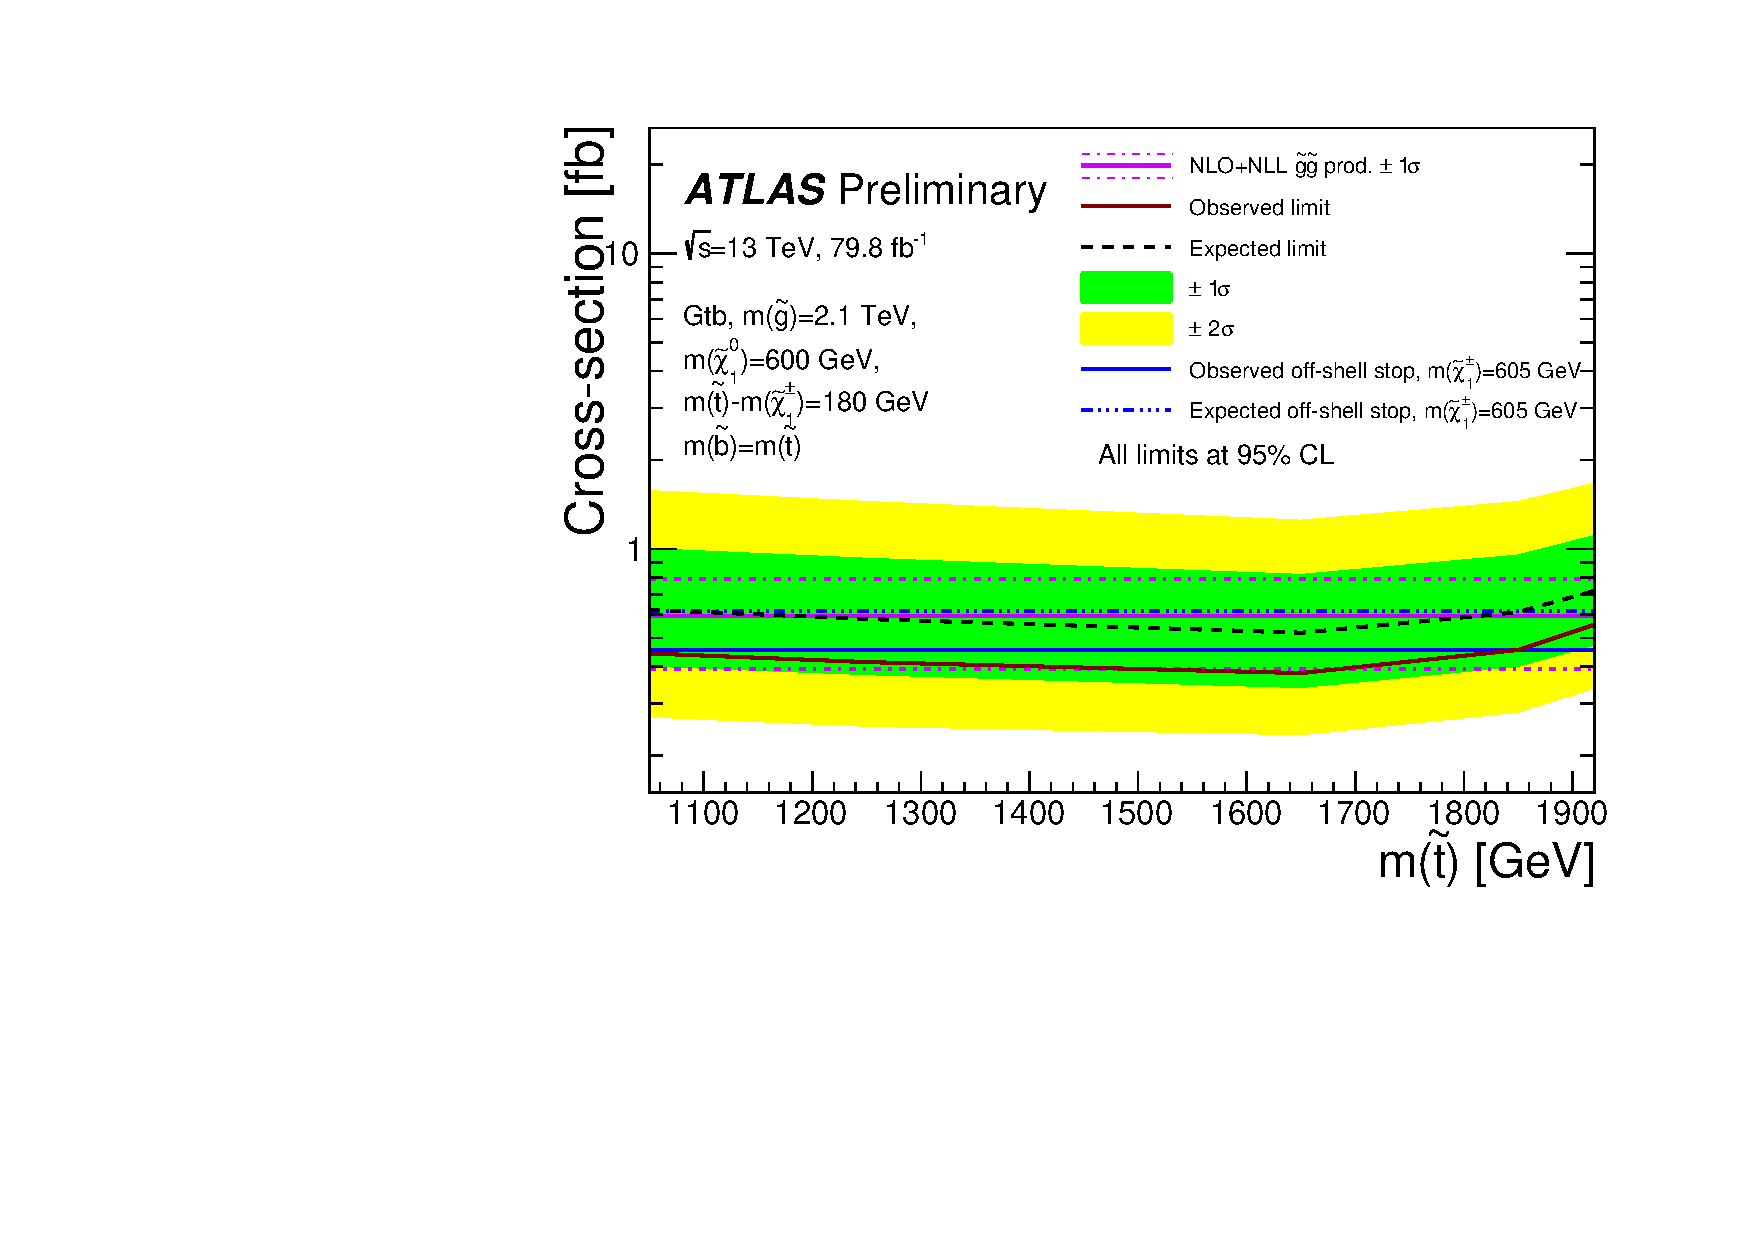
\includegraphics[width=0.75\textwidth]{figures/strong_prod/R21/multibin/Gtb_2100_diff180_600_onshell}\label{fig:limits_GtbOnshell_diff180}}
  \caption{Exclusion limits as a function of $m(\tilde{t})$, in the Gtb model but with an on-shell stop and $\chinoonepm$, 
  for $\chinoonepm$ mass fixed to 1.2 TeV \subref{fig:limits_GtbOnshell_1200} and 180 GeV lower than the stop mass \subref{fig:limits_GtbOnshell_diff180},
  in the context of the multi-bin analysis. The $\tilde{g}$ and \ninoone masses are fixed to 2.1 TeV and 600 GeV respectively.   
  The dashed and solid bold lines  show the 95\% CL expected and observed limits, respectively.    
  The solid red line indicates the theoretical cross-section for a 2.1 TeV gluino. 
  The thin blue lines indicate the expected (dashed) and observed (solid) limits for the case of the off-shell stop, where $m(\tilde{t}) = 5$ TeV, and $m(\chinoonepm) = 605$ GeV.
  Figures from Ref. \cite{ATLAS-CONF-2018-041}.}
  \label{fig:limits_GtbOnshell}
\end{figure}
